\section{Process Models}
%Providing process models is not enough because the process owner is diffident with any result which he/she is simply provided with. Therefore, he/she wants evidence of the goodness of these models. For this purpose, you should perform alignment-based conformance checking. Using the result of the conformance checker, you should motivate why the chosen models are better that any possible alternative (e.g. because of mediating fitness, precision, generalization and simplicity). For each model, also provide its textual description. 

\subsection{Exploring process}

For exploring a good model of a data set I first filtered the data with the (\textbf{Filter log on event attribute names}) tool for extracting the required. Then I used \textbf{Interactive data heuristic miner} and \textbf{Inductive Miner} on the filtered data set to discover different models. After comparing the outcomes I decided to concentrate on \textbf{Interactive data heuristic miner} and their directly followed graphs and petri nets for understanding the lifecycle. I think the petri net is the best with basic configuration and just different frequency filters. The conformance checking where done with \textbf{Replay a log on Petri Net for conformance analysis} tool on the petri net and the filtered data. For the precision check I applied the \textbf{Multi-perspective Process Explorer} tool on the petri net and the filtered data and chose "show precision mode" in the tool with basic configuration.

\subsection{Application data set}
%filter on event names
%interactive data heuristic miner oder inductive minder und dann petri net
%conformance 
%multi-perspective
Just the events beginning with "App\_..." are required. The resulting data set is saved as "Filtered App".

\subsubsection{General details of the data set}

The data set is collected between the 1st of 0ct 2011 (Saturday), 00:38:44 and the 14th of Mar 2012 (Wednesday), 15:33:57. It contains 13087 cases with 60849 executed events.

10 different events appear (occurences relative), all events are complete so I deleted this extra information: "App\_Fully\_Submission" (21.507\%), "App\_Incomplete\_Submission" (21.507\%), "App\_Rejection" (12.547\%), "App\_Pre\_Acceptation" (12.107\%), "App\_Acceptation" (8.403\%), "App\_Finalization" (8.242\%), "App\_Cancellation" (4.613\%), "App\_Initiation" (3.691\%), "App\_Approving" (3.691\%) and "App\_Registration" (3.691\%). Just "APP\_Fully\_Submission" appears to be a start event. However there are 8 end events possible: "App\_Rejection" (58.34\%), "App\_Cancellation" (21.449\%), "App\_Initiation" (8.573\%), "App\_Registration" (6.014\%), "App\_Approving" (2.575\%), "App\_Finalization" (2.499\%), "App\_Pre\_Acceptation" (0.527\%) and "App\_Acceptation" (0.023\%).


A trace contains maximal 8 different events and minimal 3. The mean is 4.65. In total there are 17 different variants of traces. 


\begin{figure}[!htbp]
\centering
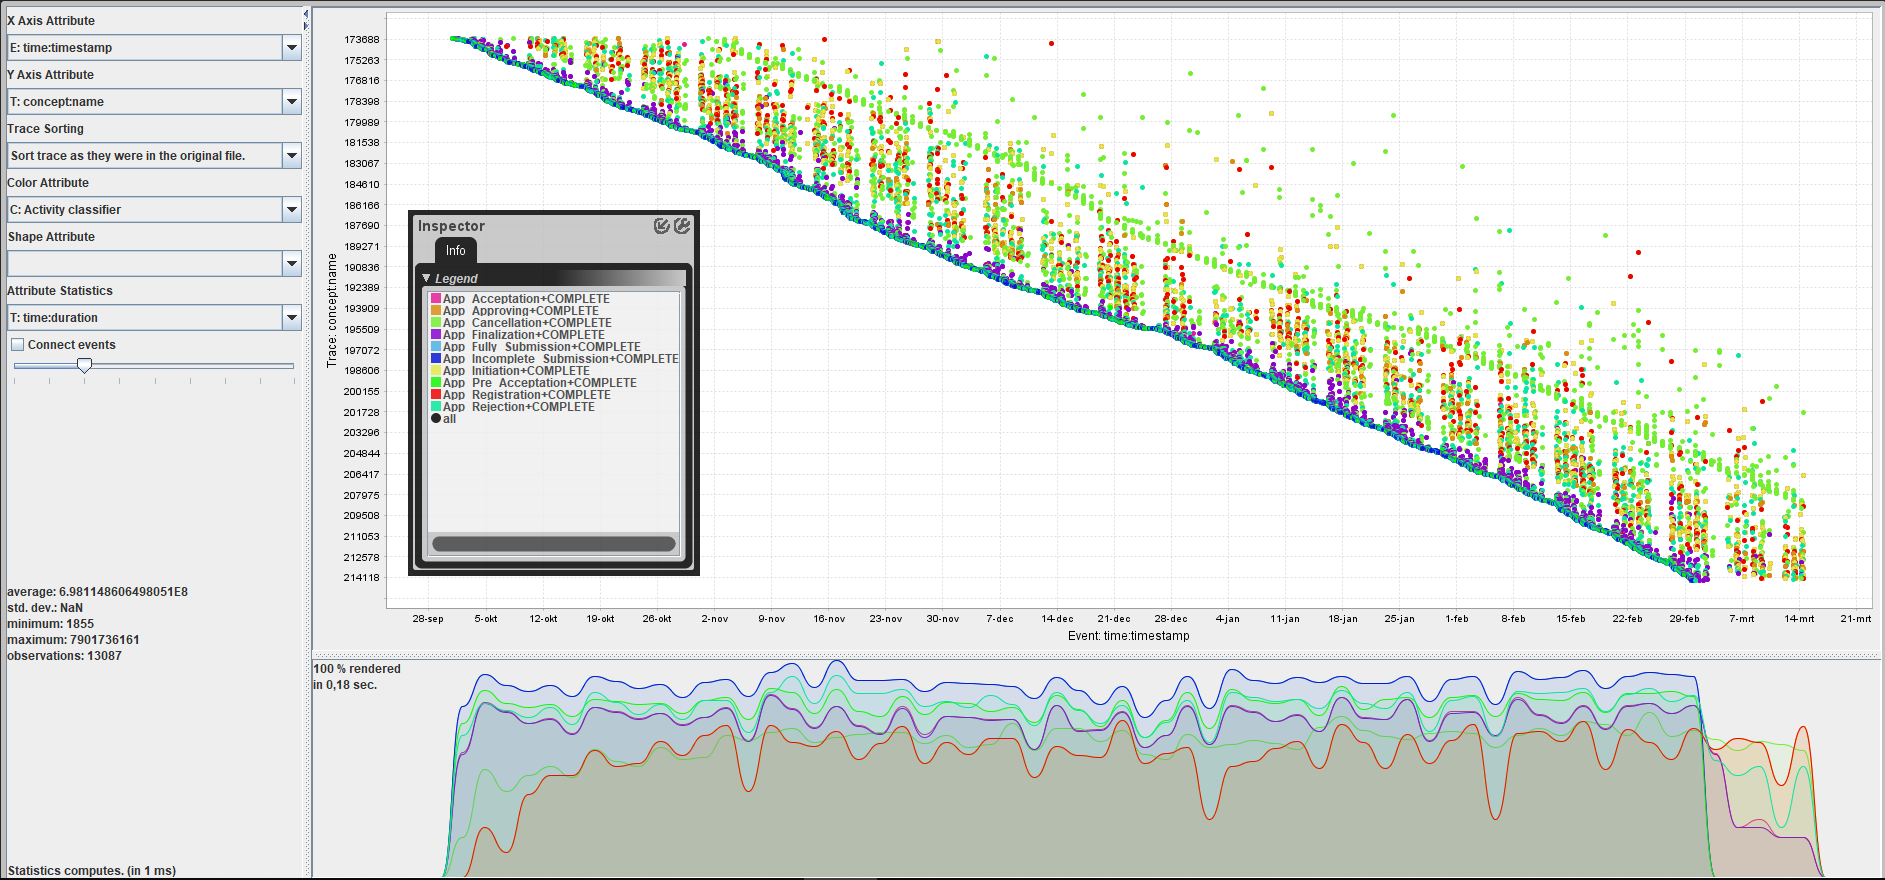
\includegraphics[height = 0.2\textheight]{AppData.PNG}
\caption{Dotted chart showing the time of events}
\label{fig:AppTimeFlow}
\end{figure}

In figure \ref{fig:AppTimeFlow} the dotted chart can be seen. Having a closer look at this chart you see gaps, which are always on a sunday. Those gaps do not appear for "APP\_Pre\_Acceptation" and "APP\_Incomplete\_Submission". Furthermore in the lower left corner the following information can be found: average duration of a case, 8 days 1 hours 55 minutes and 14.86 seconds, and the maximum duration, 91 days 10 hours 55 minutes and 36.16 seconds. Both are given in milliseconds.


\subsubsection{Discover and evaluate models of the application lifecycle}

\begin{figure}[!htbp]
\centering
\begin{subfigure}{.4\textwidth}
  \centering
  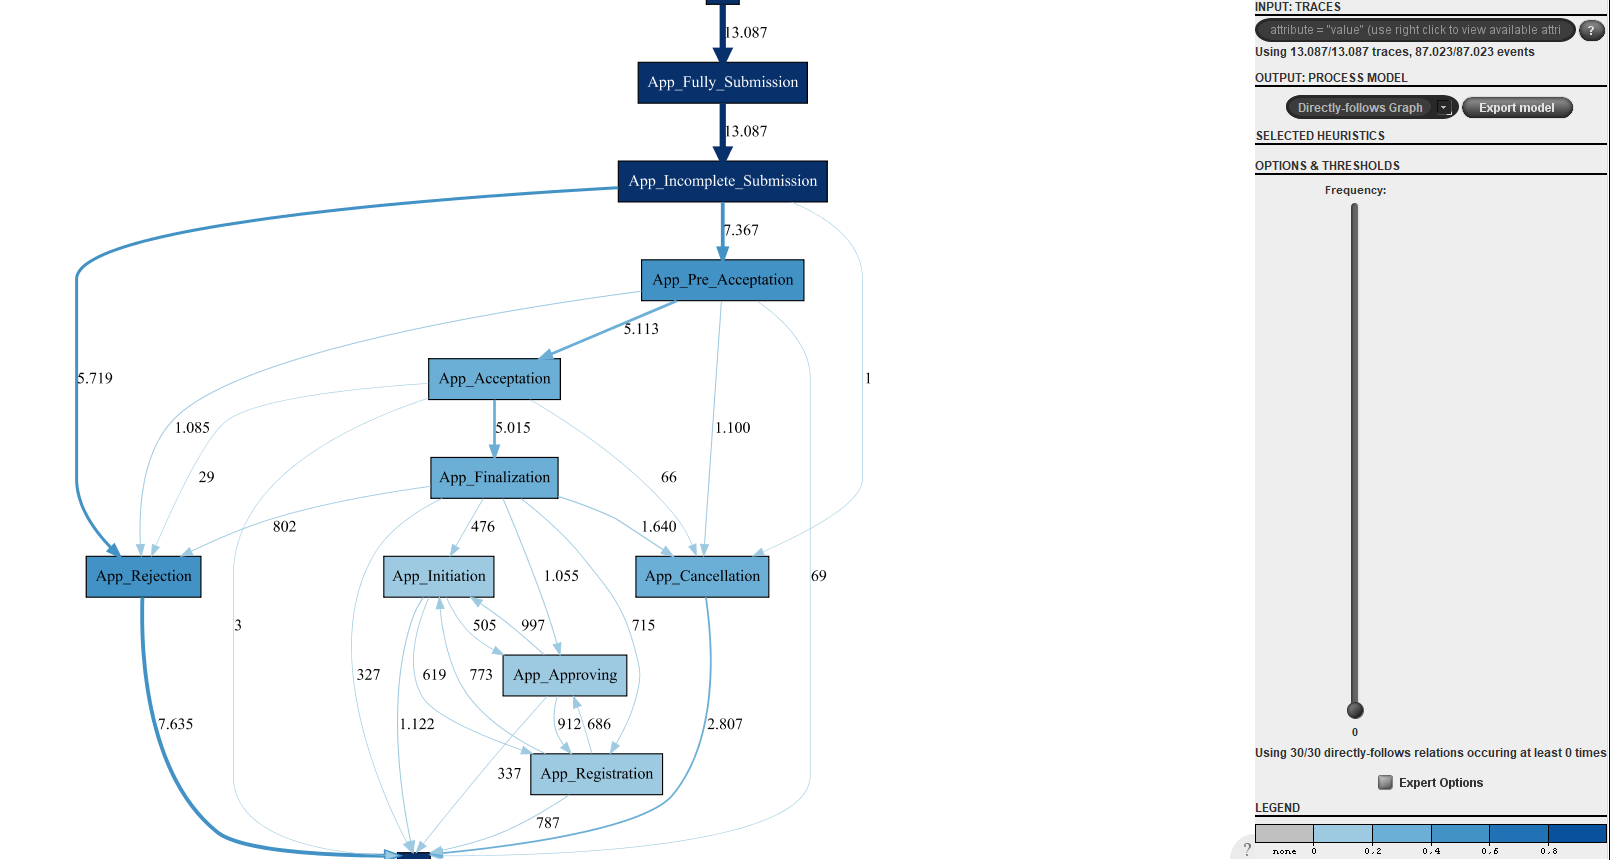
\includegraphics[width=\linewidth]{App_DirectlyFollowedFreq0.PNG}
  \caption{Petri net without frequency filtering}
  \label{fig:APP_DFG0}
\end{subfigure}%
\begin{subfigure}{.4\textwidth}
  \centering
  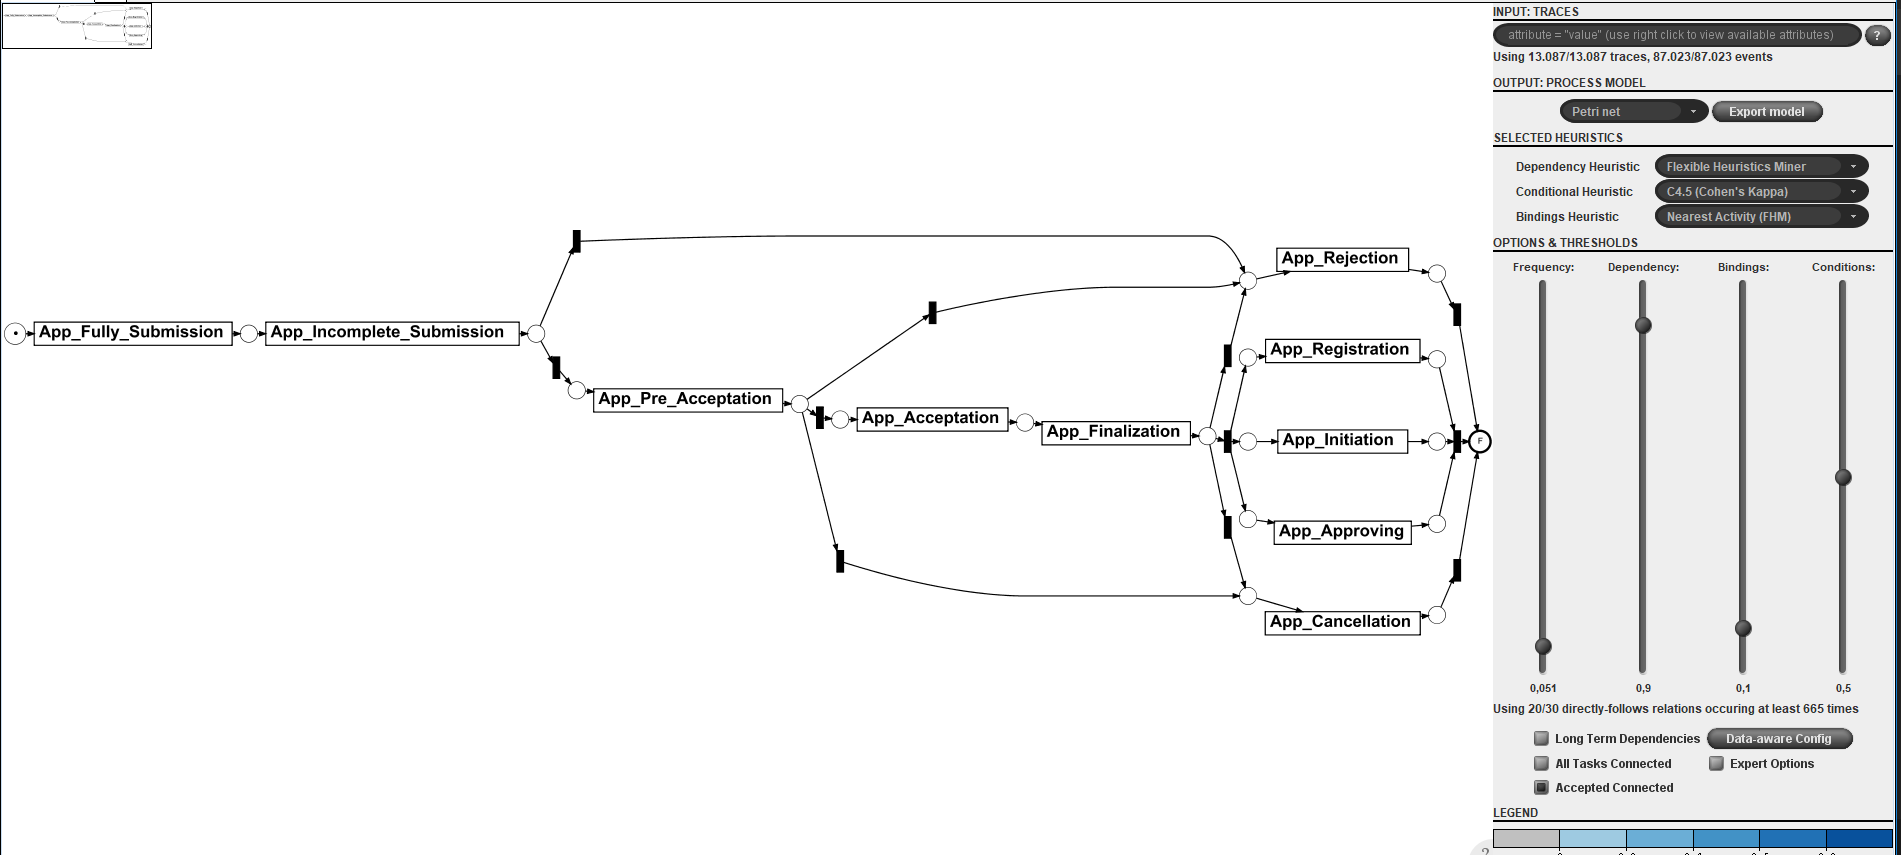
\includegraphics[width=\linewidth]{App_DirectlyFollowedFreq0-051.PNG}
  \caption{Petri net with 0.051 frequency filter}
  \label{fig:APP_DFG0-51}
\end{subfigure}
\begin{subfigure}{.4\textwidth}
  \centering
  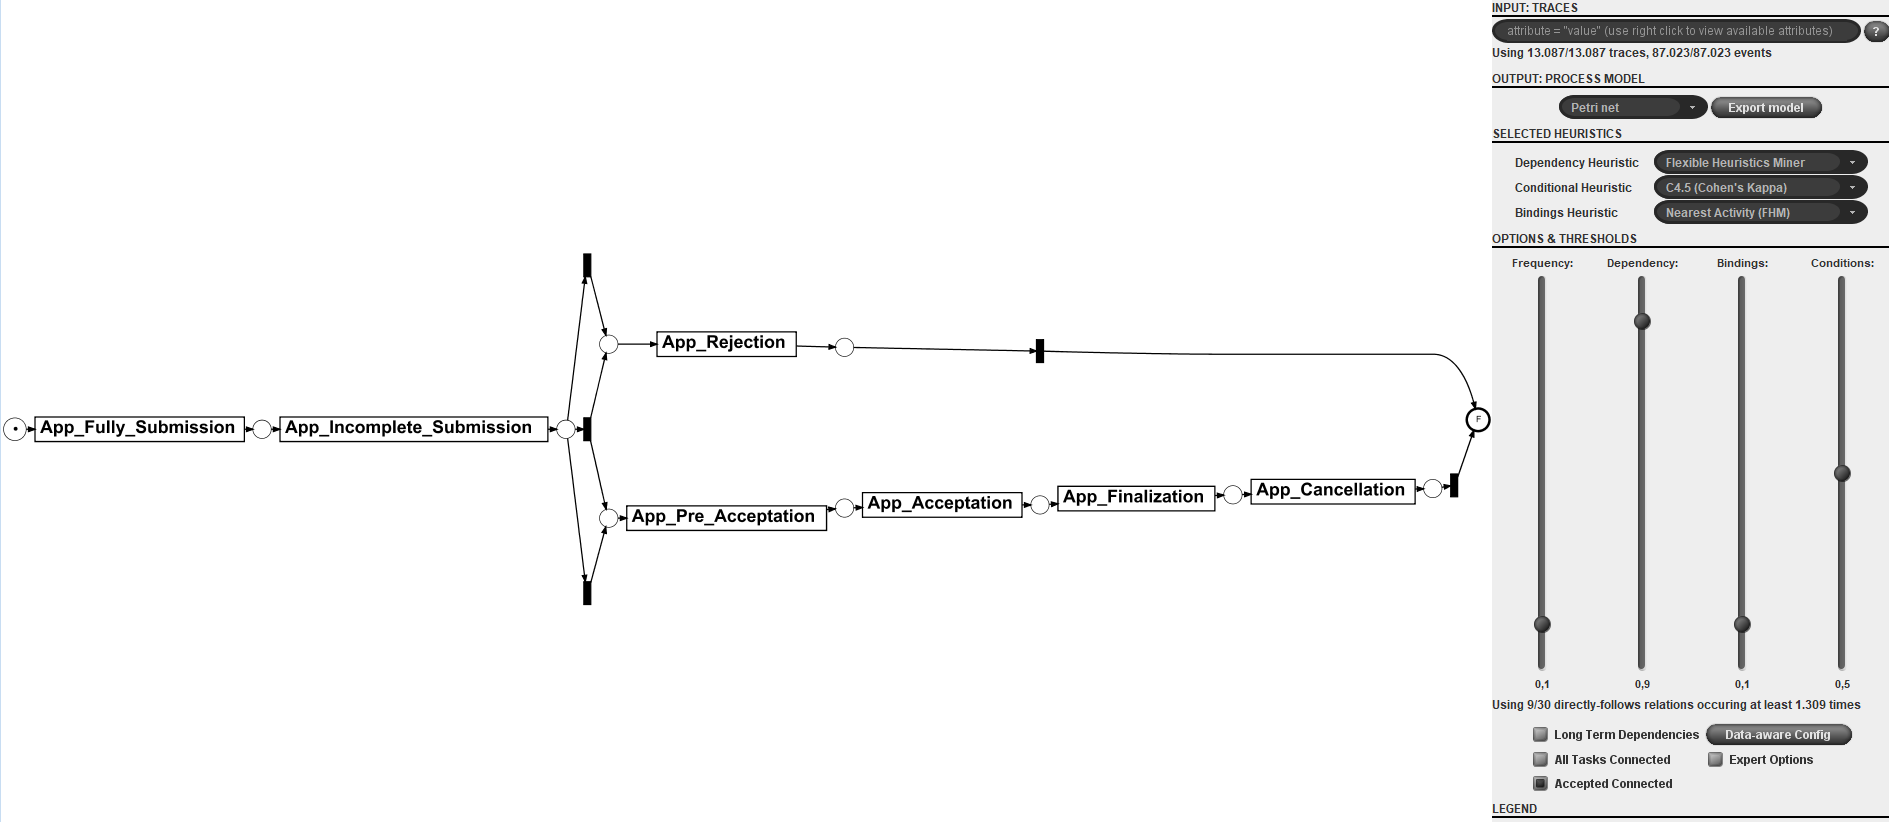
\includegraphics[width=\linewidth]{App_DirectlyFollowedFreq0-1.PNG}
  \caption{Petri net with 0.1 frequency filter}
  \label{fig:APP_DFG0-1}
\end{subfigure}
\begin{subfigure}{.4\textwidth}
  \centering
  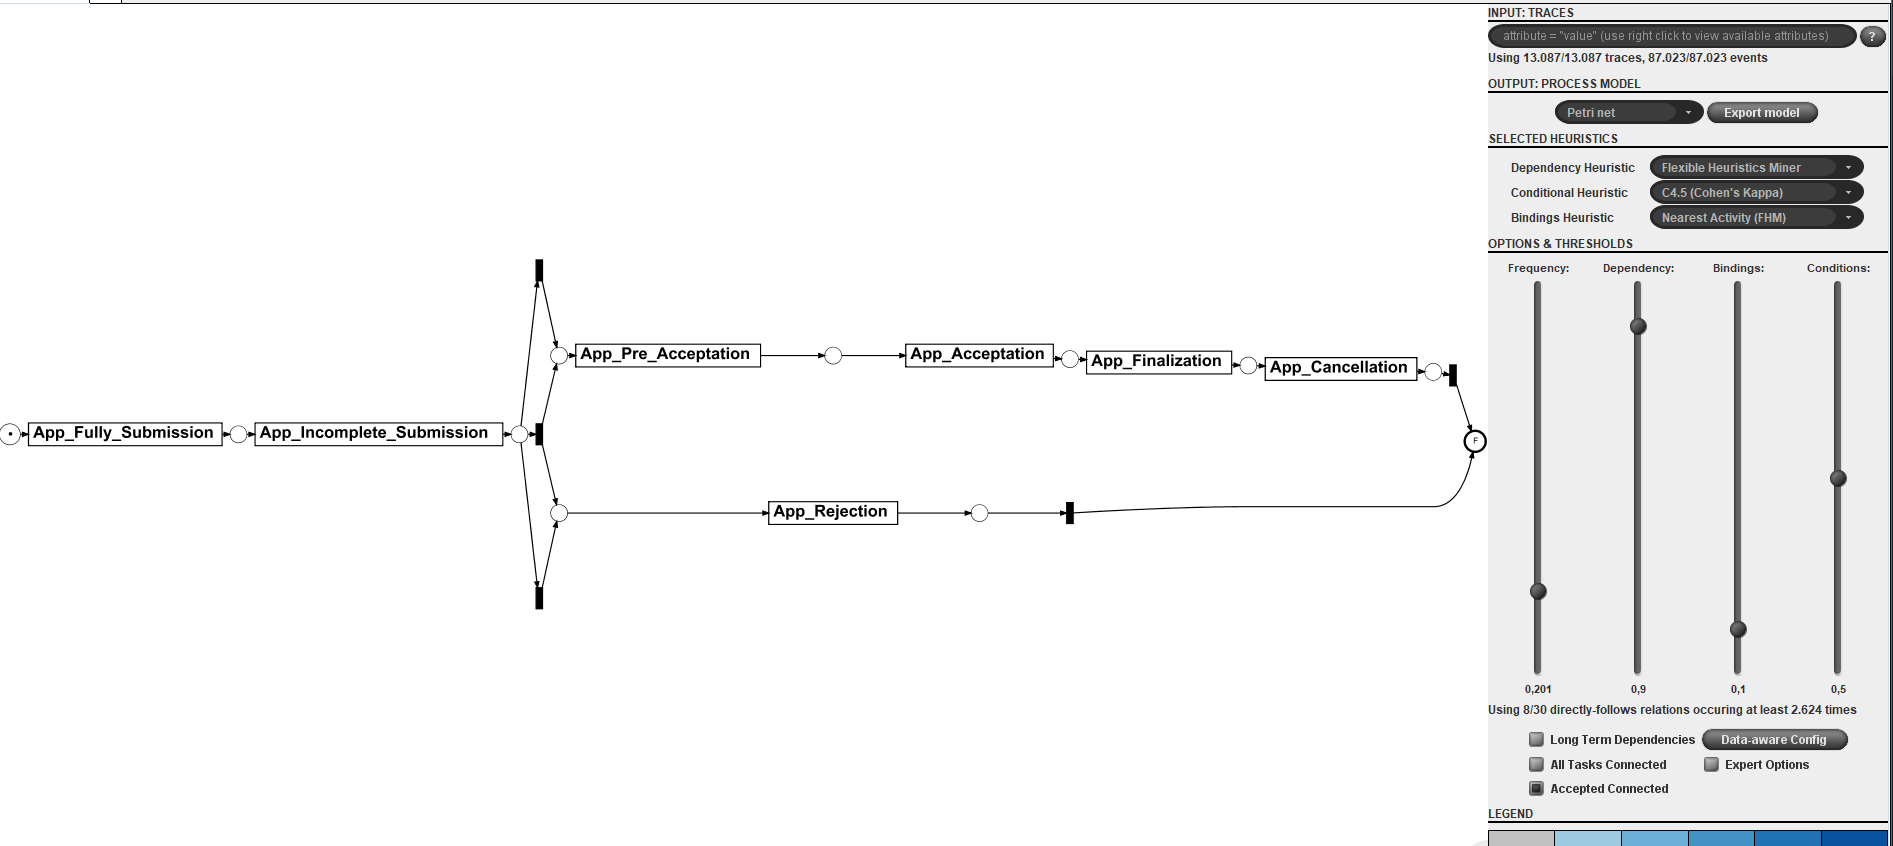
\includegraphics[width=\linewidth]{App_DirectlyFollowedFreq0-2.PNG}
  \caption{Petri net with 0.2 frequency filter}
  \label{fig:APP_DFG0-2}
\end{subfigure}
\caption{Considered petri nets}
\label{fig:App_Direct}
\end{figure}

To find an accurate model I tried different frequency filters, \ref{fig:App_Direct}. First I chose the frequency 0.1 and had a look at the resulting petri net. I also checked 0.2 and 0.51 to get a better understanding of the model(not shown here is the petri net with 0.6 filtering, which was the next filtering after 0.1, that changed the net, but I decided, that it does not contain enough cases). For comparsion in the end I had also a look at the original petri net found by the \textbf{Interactive data heuristic miner}. In figure \ref{fig:App_Direct} the 4 considered petri nets can be seen. My first choice was the petri net with 0.1 as threshold for frequency, because it was a simple model that still tells us a lot about the main process (90\% of the cases) and is not too specific (still has an acceptable generalization). Obviously the original graph does not fullfill the criterium of simplicity and also the graph with frequency 0.051 still looks not as simple. I do not consider the 0.2 filtering in the next steps, because it is the same petri net as the 0.1 filtered one.

\begin{figure}[!htbp]
\centering
\begin{subfigure}{.25\textwidth}
  \centering
  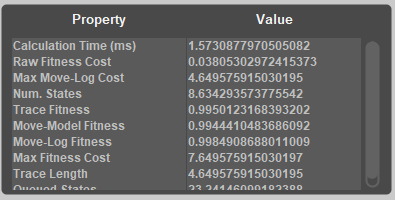
\includegraphics[width=\linewidth]{App_Conformance0-051.PNG}
  \caption{Conformance for 0.051 frequency filter}
  \label{fig:APP_Conf0-051}
\end{subfigure}%
\begin{subfigure}{.25\textwidth}
  \centering
  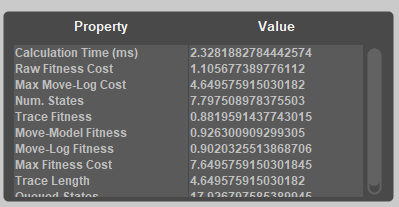
\includegraphics[width=\linewidth]{App_Conformance0-1.PNG}
  \caption{Conformance for 0.1 frequency filter}
  \label{fig:APP_Conf0-1}
\end{subfigure}
\caption{Conformance checking}
\label{fig:App_Conf}
\end{figure}


The results of the conformance checking are shown in figure \ref{fig:App_Conf}.

\begin{figure}[!htbp]
\centering
\begin{subfigure}{.4\textwidth}
  \centering
  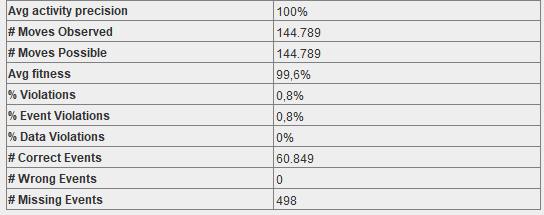
\includegraphics[width=\linewidth]{App_Precision0-051.PNG}
  \caption{Precision for 0.051 as frequency filter}
  \label{fig:APP_Prec0-051}
\end{subfigure}%
\begin{subfigure}{.4\textwidth}
  \centering
  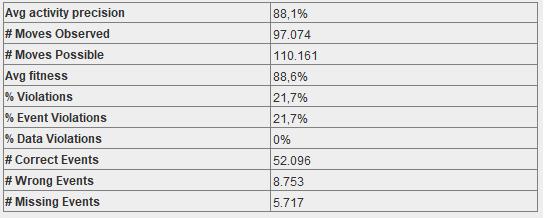
\includegraphics[width=\linewidth]{App_Precision0-1.PNG}
  \caption{Precision for 0.1 as frequency filter}
  \label{fig:APP_Prec0-1}
\end{subfigure}
\caption{Precision checking}
\label{fig:App_Prec}
\end{figure}

\begin{figure}[!htbp]
\centering
\begin{subfigure}{.9\textwidth}
  \centering
  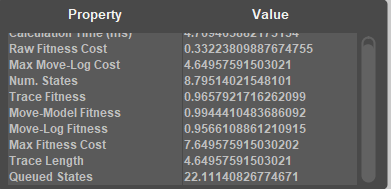
\includegraphics[width=0.4\linewidth]{App_Conformance0-069.PNG}
  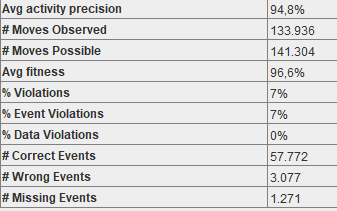
\includegraphics[width=0.4\linewidth]{App_Precision0-069.PNG}
  \caption{Conformance and Precision}
  \label{fig:APP_Conf0-069}
\end{subfigure}
\begin{subfigure}{\textwidth}
  \centering
  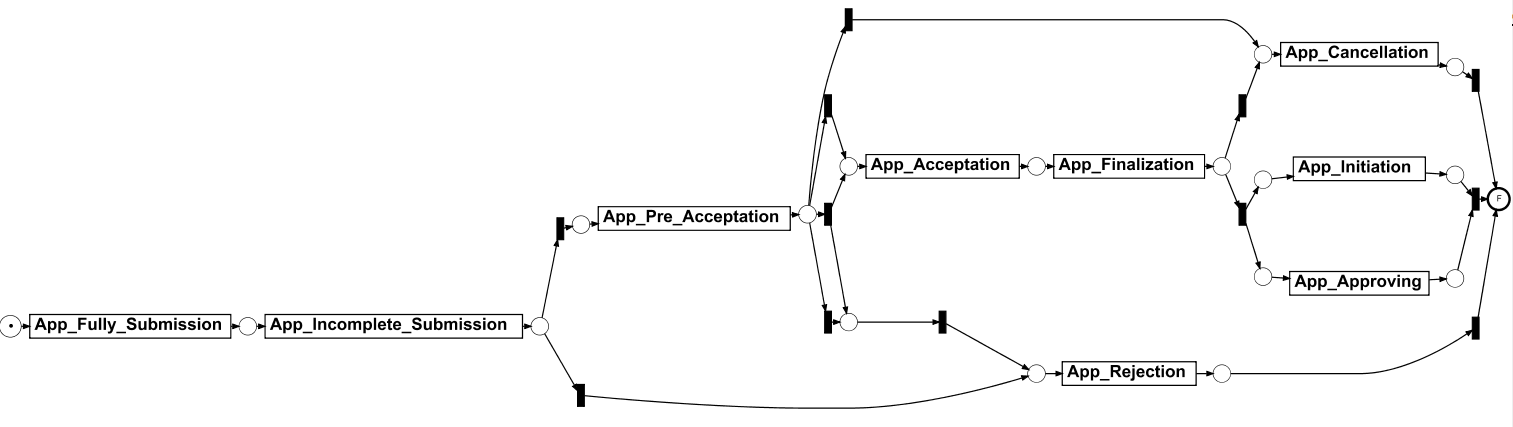
\includegraphics[width=0.9\linewidth]{App_DirectlyFollowedFreq0-069.PNG}
  \caption{Petri net}
  \label{fig:APP_DF0-069}
\end{subfigure}%
\caption{Frequency 0.069}
\label{fig:App_End}
\end{figure}
%0.07
Having a look at the precision, figure \ref{fig:App_Prec}, I could see, that the precision of 0.051 filtering is 100\%, but of the 0.1 filtering just 88.1\%. In combination with the results before, I came to the conclusion, that 0.1 filtering is not good enough as model and 0.051 would be good enough, but did not fullfill my simplicity criterium complete. Starting by 0.051 for filtering I again tried different frequency filters starting by 0.075 to find a model with a similar simplicity as the 0.1 frequency model, but a better conformance and precision than this simpel model. The best result I found was with 0.069 filtering. This model is simpel enough to understand the main lifecycle, but still has good result for conformance (fitness 96.58\%) and precision(94.8\%),\ref{fig:App_End}.
Based on this I decided to choose this petri net for the lifecycle of the application data.

\subsubsection{Discussion of the lifecycle}
Simplifying the discussion I will not write "App\_.." in begin of all events, but every event mentioned in this section is from the application data set.
\begin{figure}[!htbp]
\centering
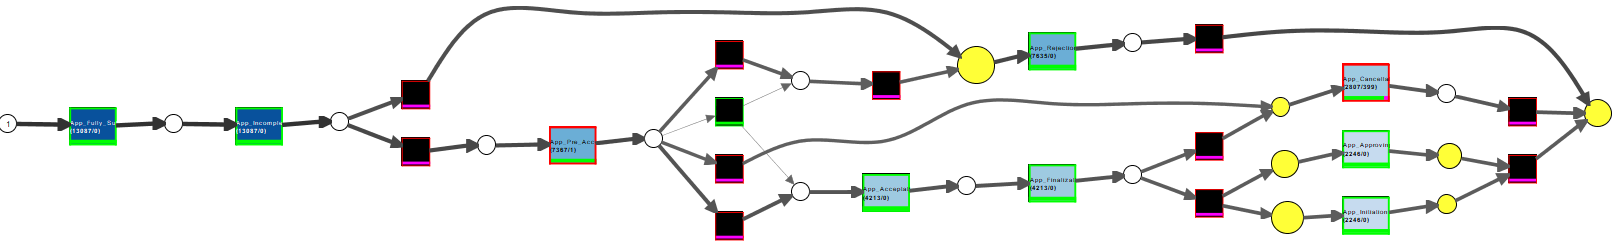
\includegraphics[width=0.9\linewidth]{APP_Replay.PNG}
\caption{Replay on petri net with 0.069 frequency filter}
\label{fig:App_EndReplay}
\end{figure}
To also have details about the occurency of the steps in the model I used the replay result, \ref{fig:App_EndReplay}.


The process always starts with "Fully\_Submission" and "Incomplete\_Submission" (13087 cases). After this there are two different outcomes:
\begin{enumerate}
	\item "Rejection" (5719 cases, executed in total in 7365 cases)
	\item "Pre\_Acceptation" (7367 cases)
\end{enumerate}

"Pre\_Acceptation" has 4 different successor events
\begin{enumerate}
	\item "Rejection" (1916 cases)
	\item "Rejection" and "Acceptation" (0 cases)
	\item "Acceptation" (4213 cases)
	\item "Cancellation" (1239 cases)
\end{enumerate}
"Acceptation" is followed by "Finalization" (4213). "Finalization" is followed in (1967 cases) by "Cancellation", which is in total executed 3206 times, and otherwise by "Approving" and Initation (2246 cases).
All the differences between incoming and outcoming cases can be explained through the filtering by frequency for building the model.

Looking at the \textbf{Time between Transition matrix} of the replay result it can be seen, that the transition to "Approving" and "Initiation" need in average \texttildelow 16 days, which is the second longest transition time. "Cancellation" has the worst transition time with in average \texttildelow 20 days.

\subsection{Proposal data}
Just the events beginning with "P\_..." are required. The resulting data set is saved as "Filtered P". Having a look in the data it was seen, that there were a lot of empty traces, so I filtered it again with the \textbf{Filter Log using Heuristics} tool, without applying any filter just everything to 100\% and saved this as "Pdoublefiltered". I use the second data set in the next steps.

\subsubsection{General Details of the data set}
The data set is collected between the 1st of 0ct 2011 (Saturday), 10:44:40 and the 14th of Mar 2012 (Wednesday), 15:50:59 and contains 5015 cases with 31244 events. Looking at the visualization you can see that there are gaps in the workflow. 

\begin{figure}[!htbp]
\centering
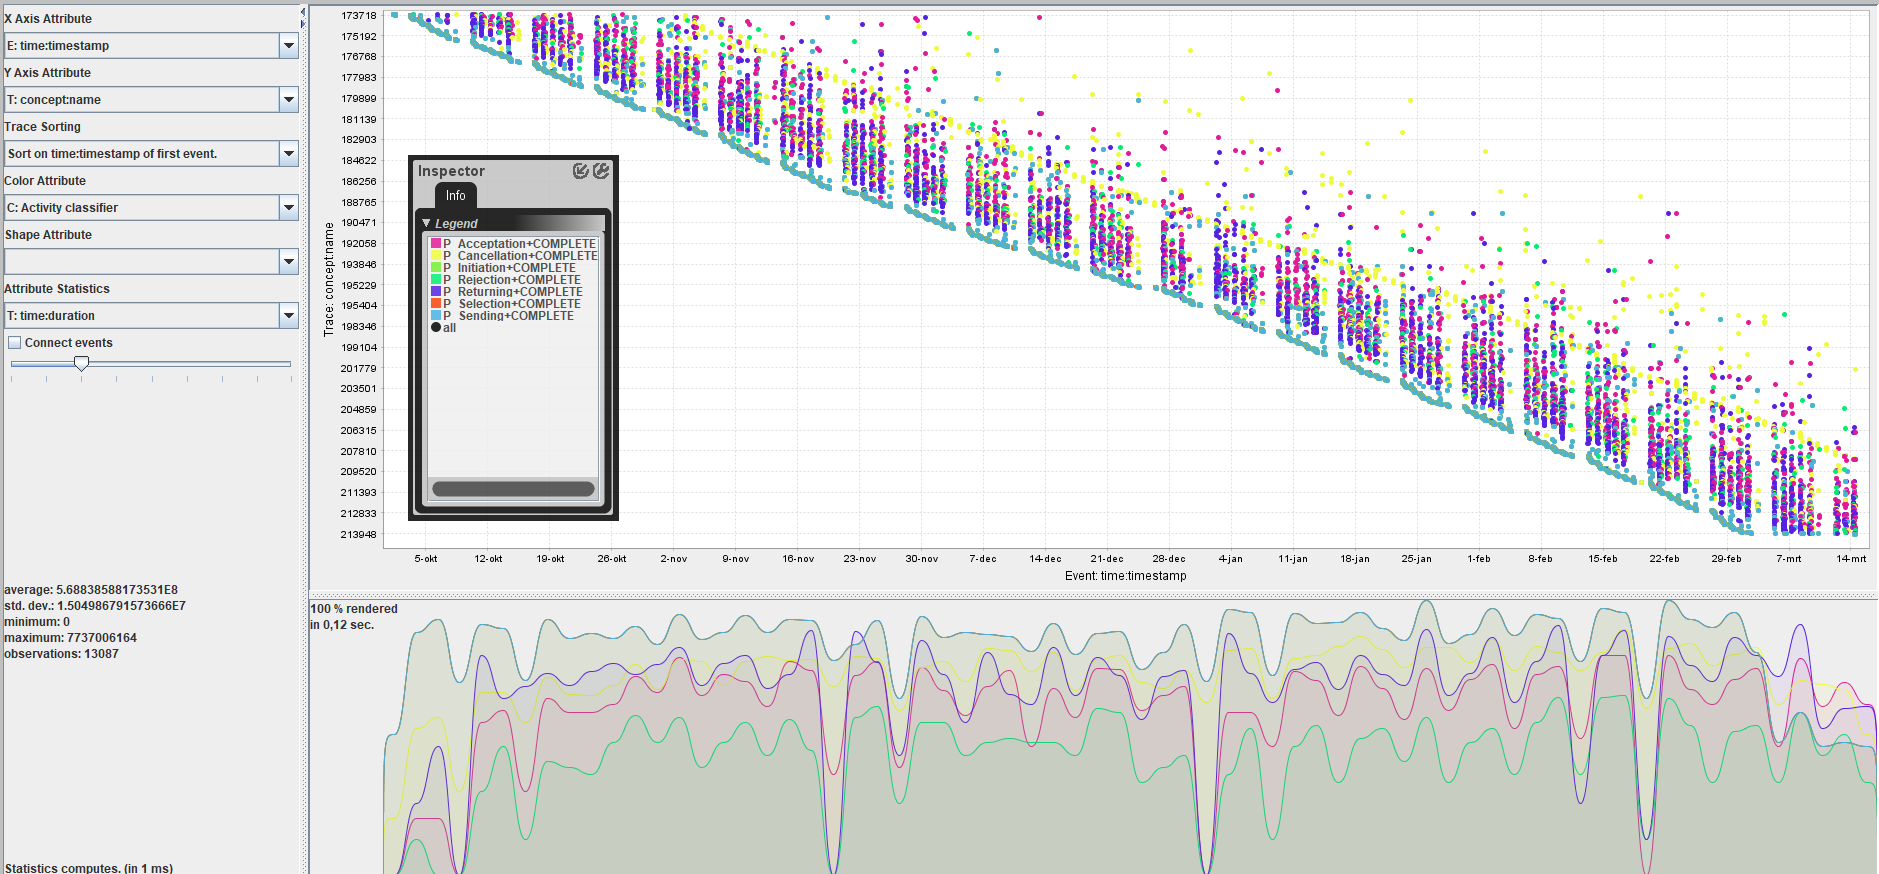
\includegraphics[height = 0.2\textheight]{ProposalData.PNG}
\caption{Dotted chart showing the time of events}
\label{fig:PropTimeFlow}
\end{figure}

In figure \ref{fig:PropTimeFlow} the dotted chart can be seen. When the gaps in the dotted chart are studied closely, it's clear that these gaps illustrate the situatioin on sundays. What does not show this behaviour so clear is "P\_Cancellation" and "P\_Initiation". Furthermore in the lower left corner the following information can be found: the average duration of a case, 17 days 4 hours 20 minutes and 24.85 seconds, the minimum duration is 667 milliseconds and the maximum duration 89 days 13 hours 10 minutes and 6.16 seconds. Both is given in milliseconds.

The data set has 7 events: 
"P\_Initiation" (22.5\%), "P\_Sending" (22.5\%), "P\_Selection" (22.5\%), "P\_Cancellation" (11.698\%), "P\_Returning" (11.055\%), "P\_Acceptation" (7.179\%) and "P\_Rejection" (2.567\%).
There are 169 different variants of traces.

All traces start with "P\_Selection". And the end events are distributed like this: 
"P\_Acceptation" (44.726\%), "P\_Cancellation" (32.702\%), "P\_Rejection" (15.992\%), "P\_Sending" (4.806\%) and "P\_Returning" (1.775\%). 

Maximal 30 events are executed in a case and minimal 3. The mean of events per class is 6.23.


\subsubsection{Discover and evaluate models of the proposal lifecycle}

Applying the steps on the proposal data set gave me in first instance 4 models I wanted to have a closer look at.

\begin{figure}[!htbp]
\centering
\begin{subfigure}{.4\textwidth}
  \centering
  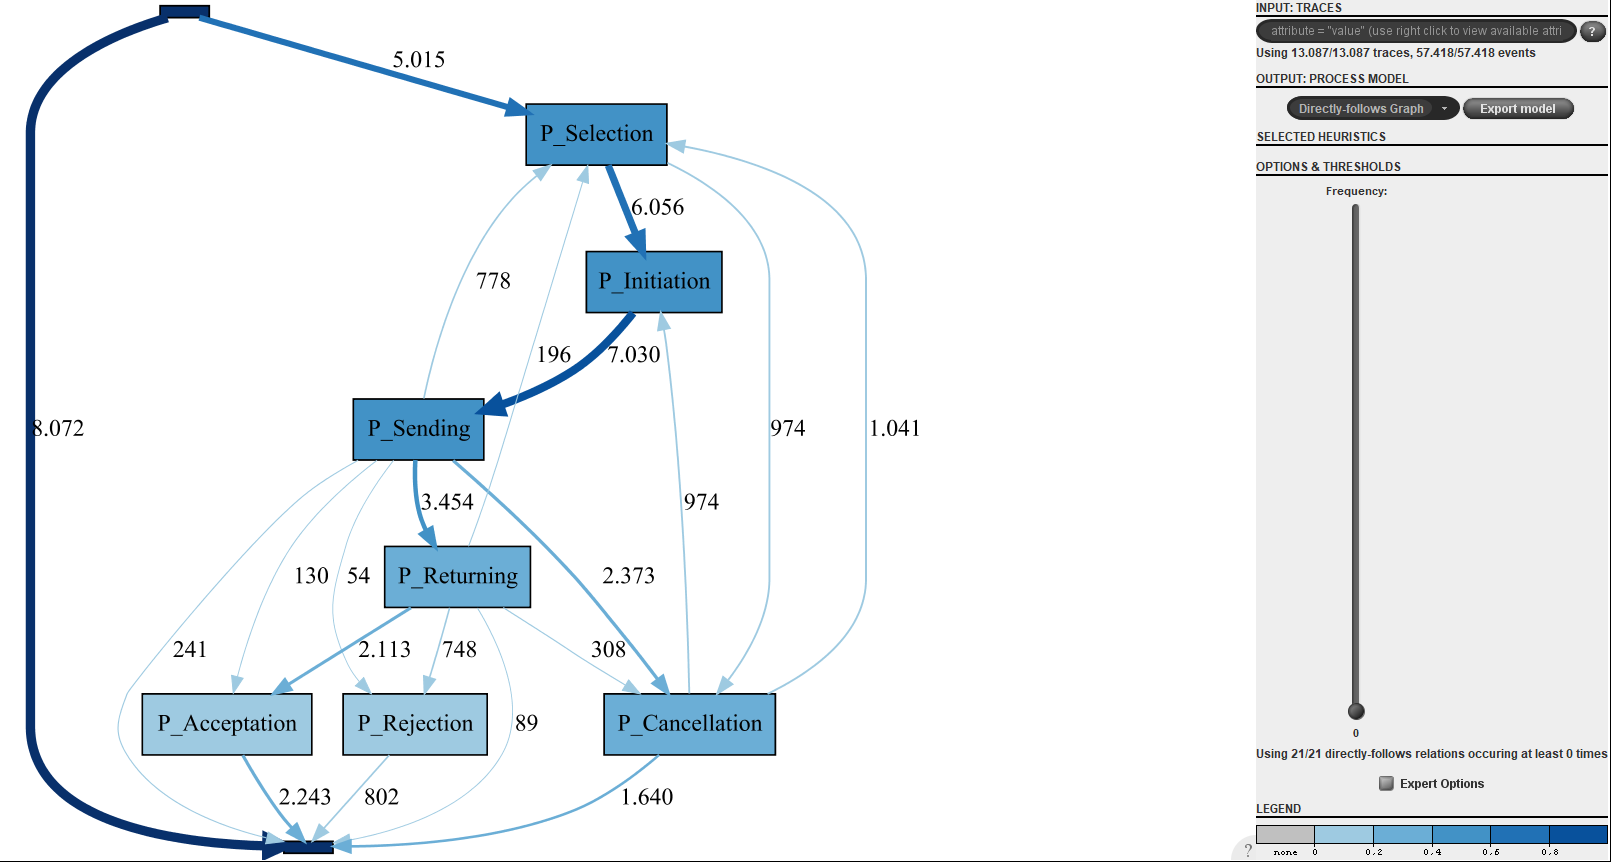
\includegraphics[width=\linewidth]{P_DirectlyFollowedFreq0.PNG}
  \caption{Petri net without frequency filtering}
  \label{fig:P_DFG0}
\end{subfigure}%
\begin{subfigure}{.4\textwidth}
  \centering
  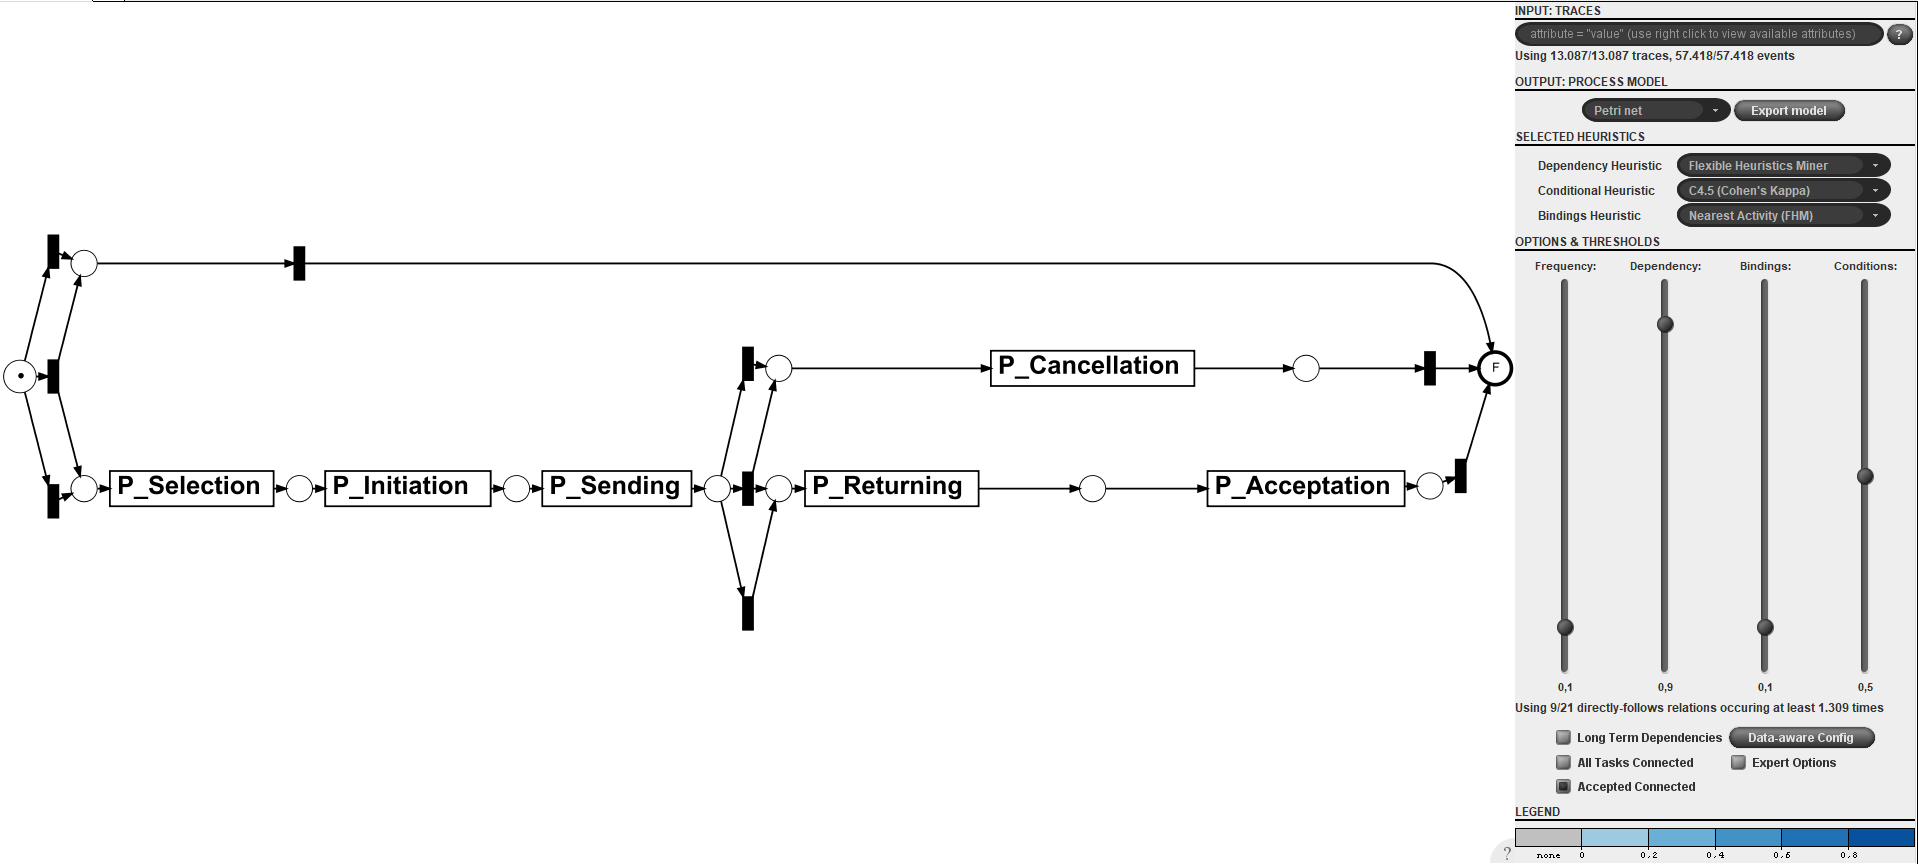
\includegraphics[width=\linewidth]{P_DirectlyFollowedFreq0-1.PNG}
  \caption{Directly followed graph 0.1 frequency filter}
  \label{fig:P_DFG0-1}
\end{subfigure}
\begin{subfigure}{.4\textwidth}
  \centering
  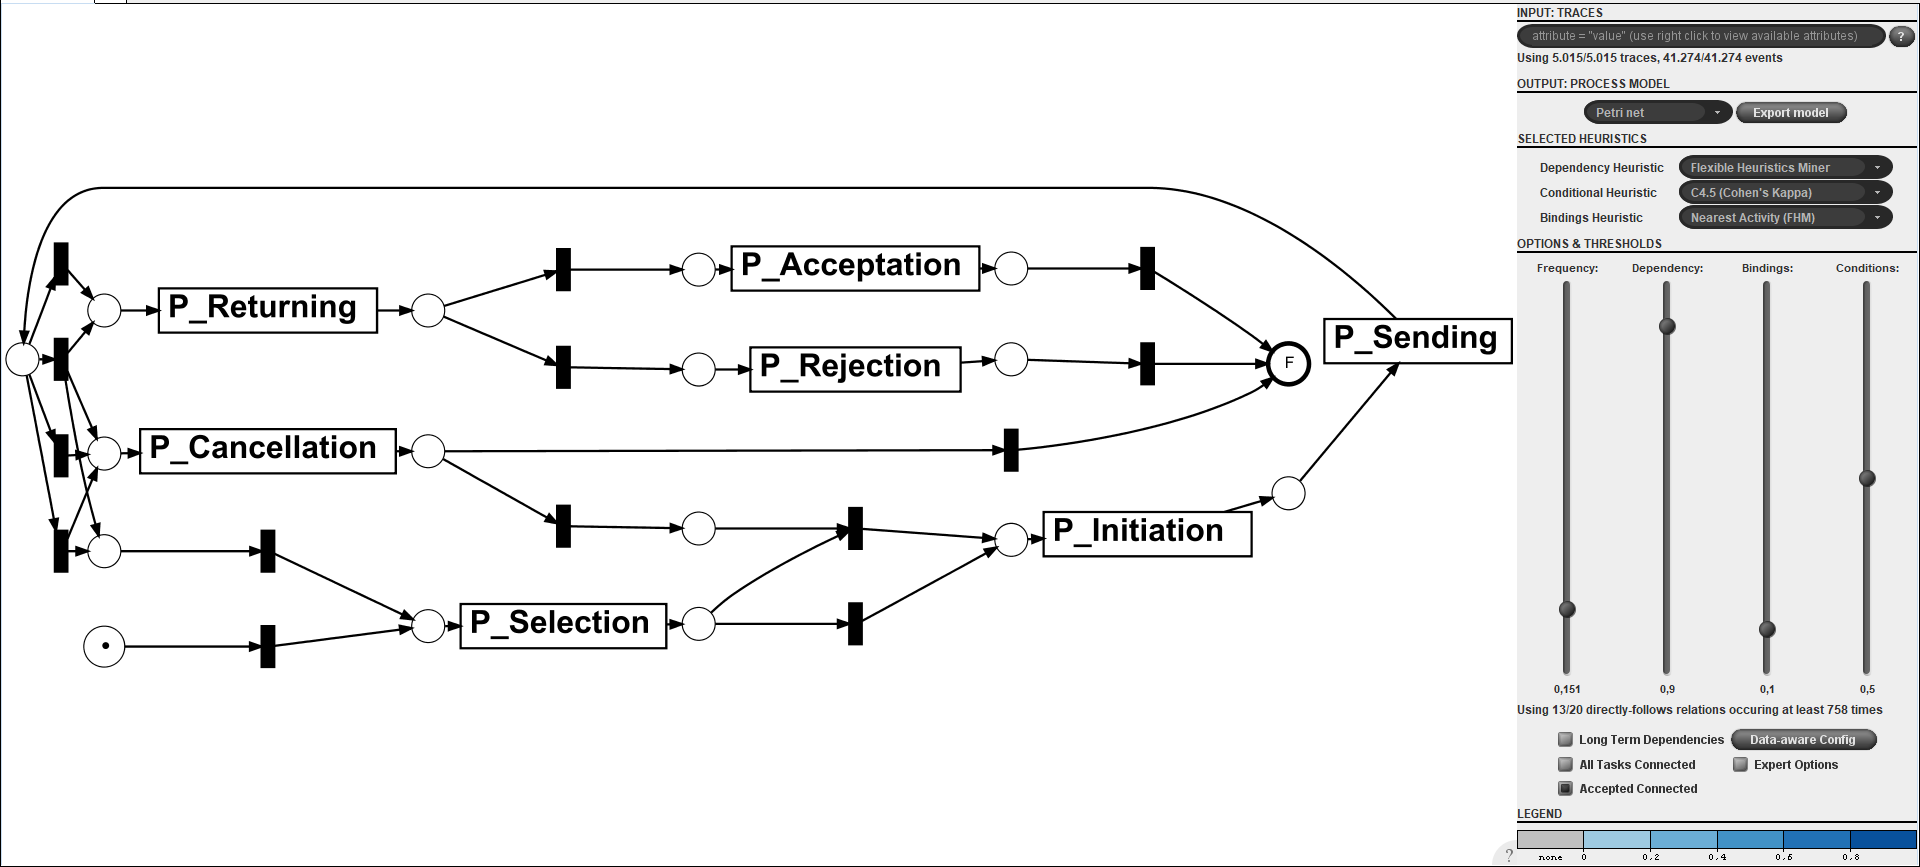
\includegraphics[width=\linewidth]{P_DirectlyFollowedFreq0-151.PNG}
  \caption{Petri net for 0.151 frequency filter}
  \label{fig:P_DFG0-151}
\end{subfigure}
\begin{subfigure}{.4\textwidth}
  \centering
  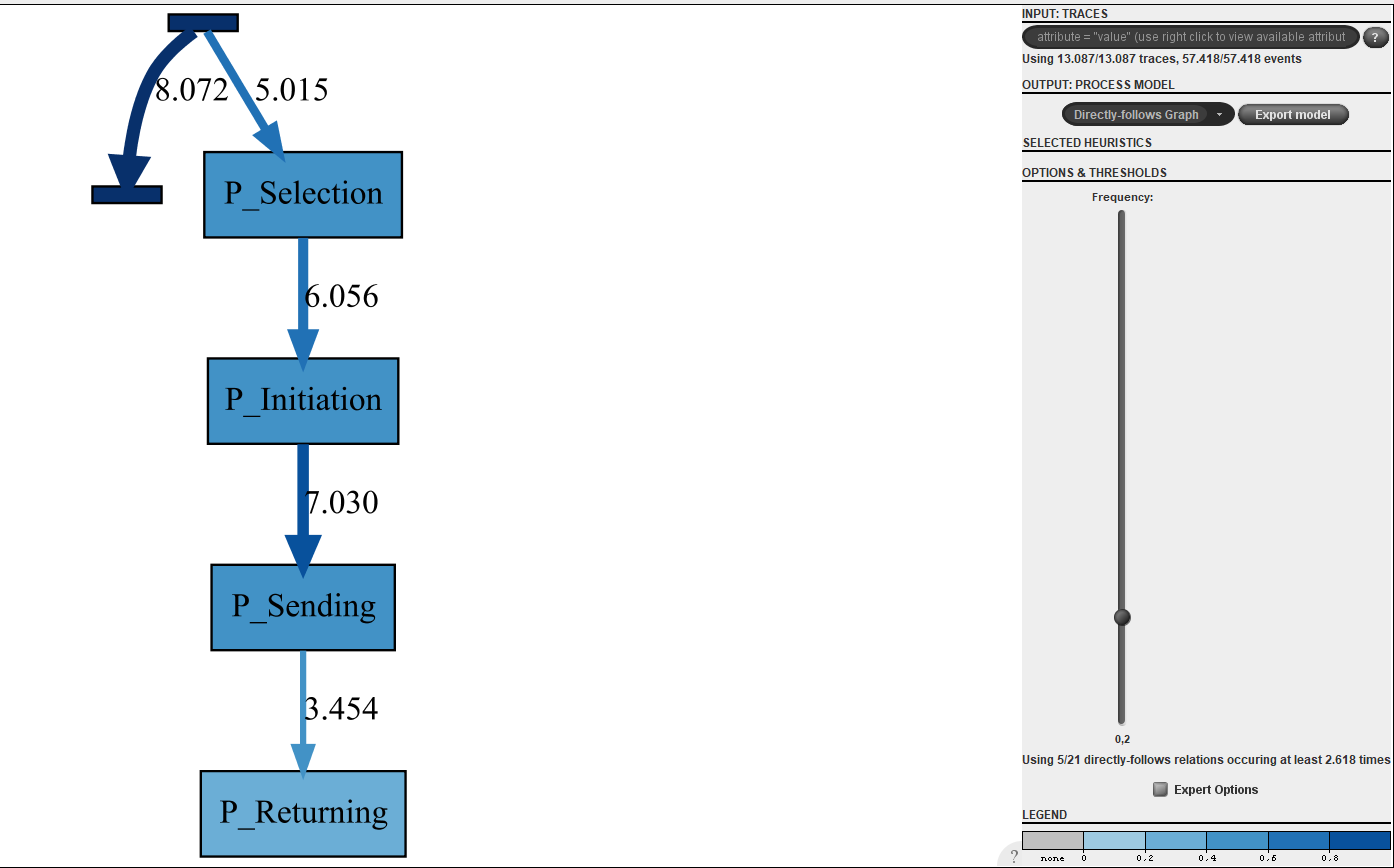
\includegraphics[width=\linewidth]{P_DirectlyFollowedFreq0-2.PNG}
  \caption{Petri net for 0.2 frequency filter}
  \label{fig:P_DFG0-2}
\end{subfigure}
\caption{Considered petri nets}
\label{fig:P_Direct}
\end{figure}

Because of simplicity reasons I picked out of those, figure \ref{fig:P_Direct}, just the 0.151 and 0.2 filtered petri nets.


\begin{figure}[!htbp]
\centering
\begin{subfigure}{.4\textwidth}
  \centering
  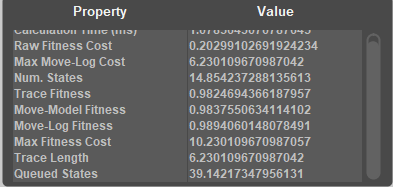
\includegraphics[width=\linewidth]{P_Conformance0-151.PNG}
  \caption{Conformance for 0.151 as frequency filter}
  \label{fig:P_Conf0-151}
\end{subfigure}%
\begin{subfigure}{.4\textwidth}
  \centering
  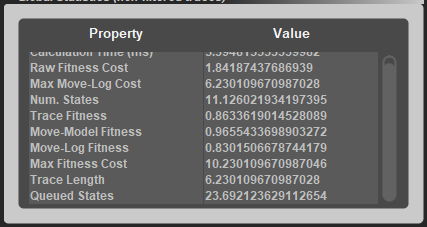
\includegraphics[width=\linewidth]{P_Conformance0-2.PNG}
  \caption{Conformance for 0.2 as frequency filter}
  \label{fig:P_Conf0-2}
\end{subfigure}
\begin{subfigure}{.4\textwidth}
  \centering
  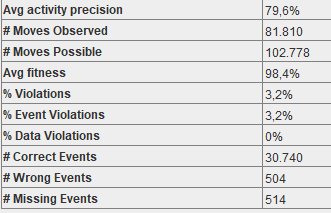
\includegraphics[width=\linewidth]{P_Precision0-151.PNG}
  \caption{Precision for 0.151 as frequency filter}
  \label{fig:P_Prec0-151}
\end{subfigure}%
\begin{subfigure}{.4\textwidth}
  \centering
  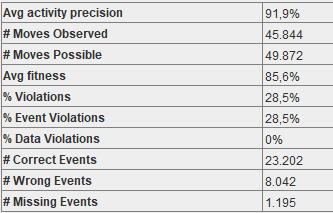
\includegraphics[width=\linewidth]{P_Precision0-2.PNG}
  \caption{Precision for 0.2 as frequency filter}
  \label{fig:P_Prec0-2}
\end{subfigure}
\caption{Conformance and precision checking}
\label{fig:P_ConfPrec}
\end{figure}


The conformance and precision outcomes(see in figure \ref{fig:P_ConfPrec}) told me, that the 0.2 frequency model (fitness 86.33\%, precision 91.9\%) has a better outcome for the precision as the 0.151 filtered model(precision 79.6\%), but a worse for the fitness (98.25\%). So I searched for an other model, which has a similar simplicity as the 0.2 and 0.151 filtered models and might have a better fitness or precision. The model fullfilling simplicity was 0.175 filtering, but the fitness was worse, than for 0.2 filtering. I tried this with several other filterings, but the best was 0.2 filtering, so I chose this one.


\subsubsection{Discussion of the lifecycle}
Simplifying the discussion I will not write "P\_.." in begin of all events, but every event mentioned in this section is from the proposal data set.

\begin{figure}[!htbp]
  \begin{center}
    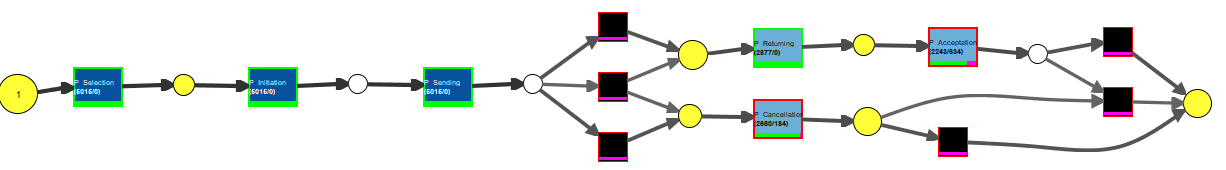
\includegraphics[width = 0.9\textwidth]{P_ConfomGraph0-2.png}
  \end{center}
  \caption{Replay on petri net with 0.2 frequency filter}
\end{figure}

5015 cases start with "Selection". Then "Initiation" event is performed (5015 cases). "Initiation" is followed by "Sending" (5015 cases), which has 3 different succesor actions. 
\begin{enumerate}
	\item "Returning" (2171 cases)
	\item "Returning" and "Cancellation" (706 times)
	\item "Cancellation"  (2138 times)
\end{enumerate}
"Returning" is in 2243 cases followed by "Acceptation". "Cancellation" and "Acceptation" have to be joined again if it was an end split before

\subsection{Combined Model}
%Models that combine these two models into one showing the lifecycle of the application and the proposal together. Due to the high variability, you should discover one different model for each possible outcome, namely whether the application is finally rejected, cancelled or approved. 

For combined Models I first filtered the data to have a dataset with all proposal data combined with the application data. This data I filtered with Heuristic filter (all configurations to 100\% and just deciding what the endstate is) with the outcomes/endstates "APP\_rejected" or "APP\_cancelled" or "APP\_approved". I saved them under the names "Filtered P App with approv", "Filtered P App with canc" and "Filtered P App with rej". 

\subsubsection{Endstate APP\_Approved}

\textbf{General Details of the data set}

The data set is collected between the 1st of 0ct 2011 (Saturday), 12:36:08 and the 14th of Mar 2012 (Wednesday), 15:23:32. The set contains 301 and 4550 events executed. 

\begin{figure}[!htbp]
\centering
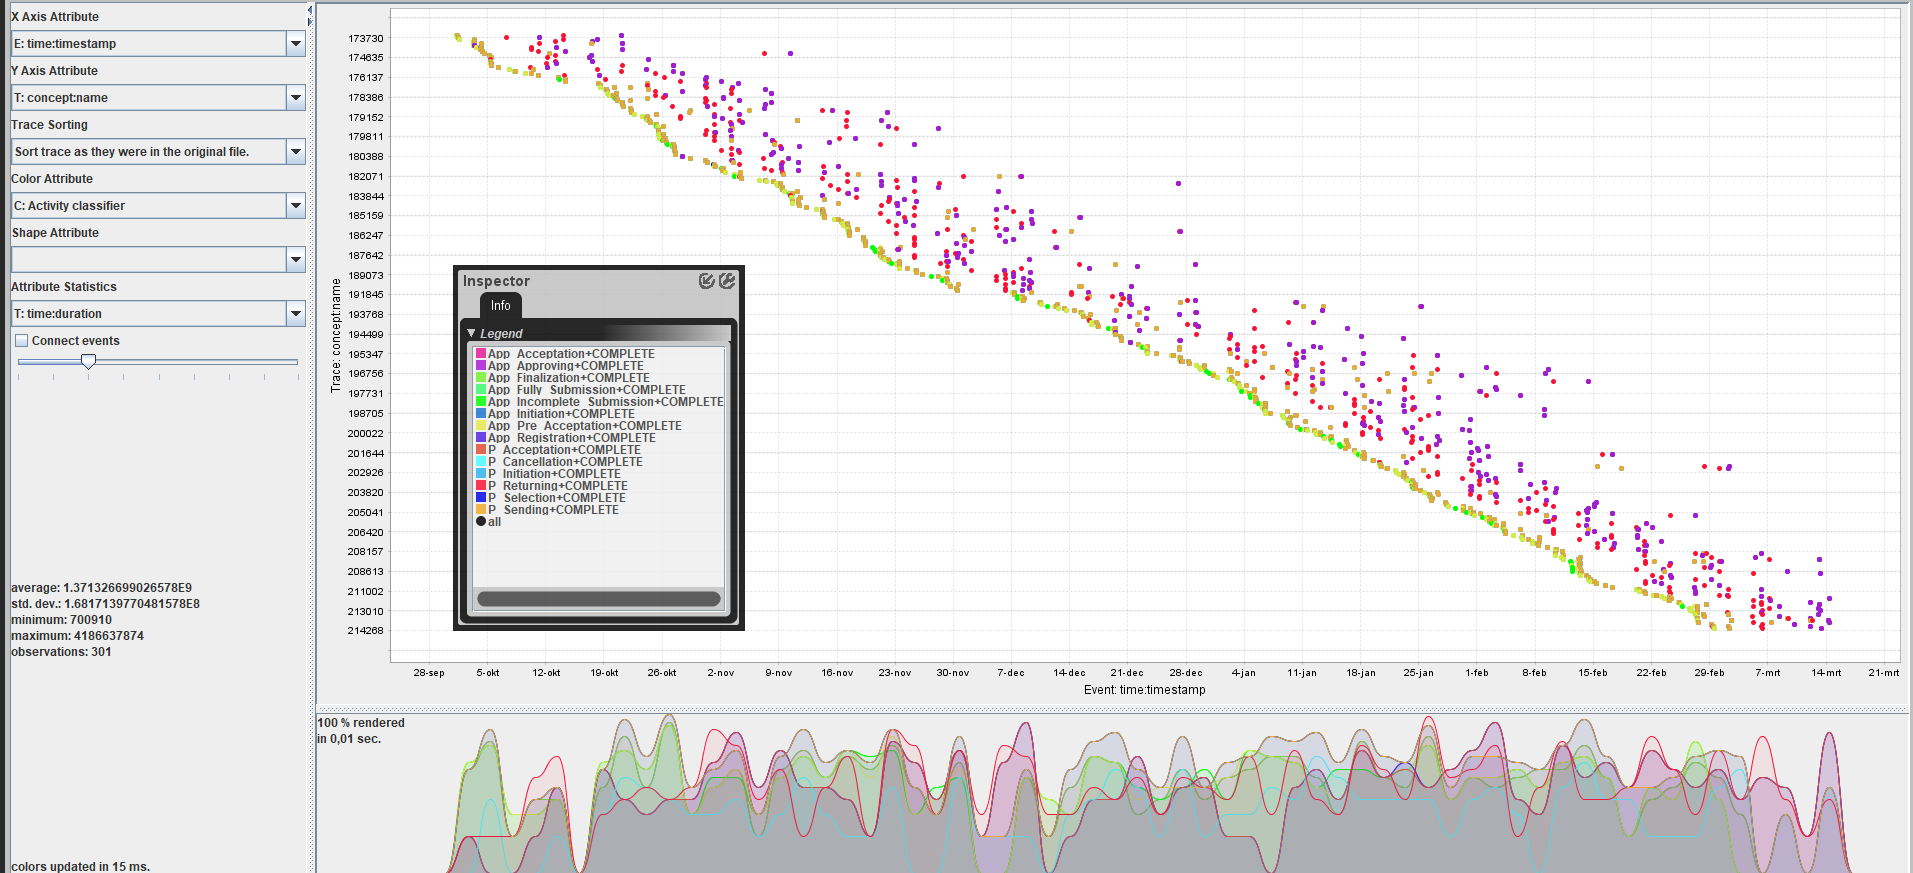
\includegraphics[height = 0.2\textheight]{ApprovalDot.PNG}
\caption{Dotted chart showing the time of events}
\label{fig:ApprovTimeFlow}
\end{figure}

In figure \ref{fig:ApprovTimeFlow} the dotted chart can be seen. There is a gap visible on every sunday. This is more clearly to see, when changing the color to days of the week. There you can see, that it is always a sunday. Furthermore in the left lower corner the following information can be found: average duration of a case is, 15 days 20 hours 55 minutes and 26.70 seconds, the minimal duration, 11 minutes and 40.91 seconds, and the maximum duration, 48 days 27 hours 23 minutes and 14.69 seconds. Those are given in milliseconds in the figure.

There are 14 different events:
"P\_Initiation" (10.0\%), "P\_Sending" (10.0\%), "P\_Selection" (10.0\%), "P\_Returning" (7.099\%), "App\_Pre\_Acceptation" (6.615\%), "App\_Initiation" (6.615\%), "App\_Approving" (6.615\%), "App\_Registration" (6.615\%), "App\_Finalization" (6.615\%), "App\_Fully\_Submission" (6.615\%), "App\_Incomplete\_Submission" (6.615\%), "App\_Acceptation" (6.615\%), "P\_Acceptation" (6.593\%), "P\_Cancellation" (3.385\%). The percentages are the relative occurences.
There are 73 different variants of traces.

All events start with "App\_Fully\_Submission".

Maximal 34 events are executed in a case and minimal 12. The mean of events per class is 15.116.


\textbf{Discover and evaluate models of lifecycle with Endstate APP\_Approved}

Like for approved and proposal I first checked different frequency filter setting to have a first idea, which models fullfill simplicity. Then for every chosen frequency in begin I checked conformance and precision.

\begin{figure}[!htbp]
\centering
\begin{tabular}{c|c|c|c|c|}
\cline{2-5}
& \multicolumn{4}{ c| }{Frequency} \\ \cline{2-5}
& 0 & 0.1 & 0.2 & 0.3 \\ \cline{1-5}
\multicolumn{1}{ |c|  }{Simplicity} 
& - & - & + & ++      \\ \cline{1-5}
\multicolumn{1}{ |c|  }{Fitness}  & 99.84 & 99.47 & 93.93 & 93.93      \\ \cline{1-5}
\multicolumn{1}{ |c| } {Precision} & 93.3 & 94.5 & 91.7 & 94.8  \\ \cline{1-5}
\end{tabular}
\caption{Results for approved as endstate}
\label{tab:ApprovRe}
\end{figure}

Based on the results, \ref{tab:ApprovRe}, I chose the model with 0.3 filtering. This one has a high simplicity, but still has surprisingly good results.
%TODO Maybe all together

\textbf{Discussion of the model}

\begin{figure}[!htbp]
\centering
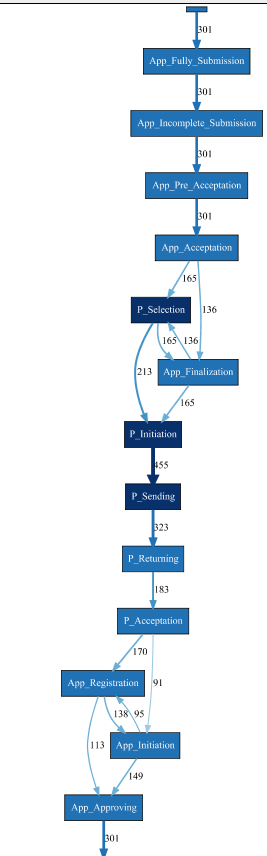
\includegraphics[width =0.9\textwidth]{APP_ApprovedDFG0-3.PNG}  
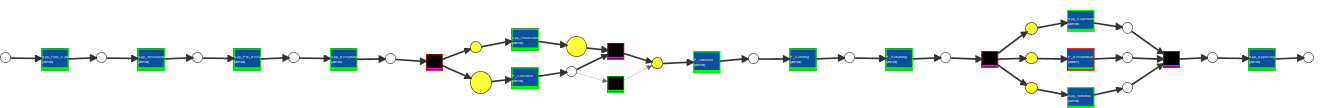
\includegraphics[width =0.9\textwidth]{ApprovReplay.PNG}
\caption{Endstate APP\_Approved}
\label{fig:ApprovModel}
\end{figure}

In figure \ref{fig:ApprovModel} the petri net and the result of the replat can be seen. It is hard to clearly read the details, but I describe it in detail here. 

All 301 cases start with the same 4 events: "App\_Fully\_Submission" \textrightarrow "App\_Incomplete\_Submission" \textrightarrow "App\_Pre\_Acceptation" \textrightarrow "App\_Acceptation". Then there are two events parallel: "App\_Finalization" and "P\_Selection". Before and after those actions are events skipped in the model, that occur in the original log. Afterwards "P\_Initiation" \textrightarrow "P\_Sending" \textrightarrow "P\_Returning" are executed in all cases. Again 3 events are parallel "App\_Registration", "App\_Registration" (just in 300 cases and "App\_Initiation". The last event is "App\_Approving".

When I controlled the time matrix for the transitions I saw, that there are a lot of transitions taking place between 12 and 16 days.

\subsubsection{Endstate APP\_Cancelled}


\textbf{General Details of the data set}

The data set is collected between the 1st of 0ct 2011 (Saturday), 09:45:25 and the 14th of Mar 2012 (Wednesday), 15:30:47. The set contains 1937 and 13524 events executed. 

\begin{figure}[!htbp]
\centering
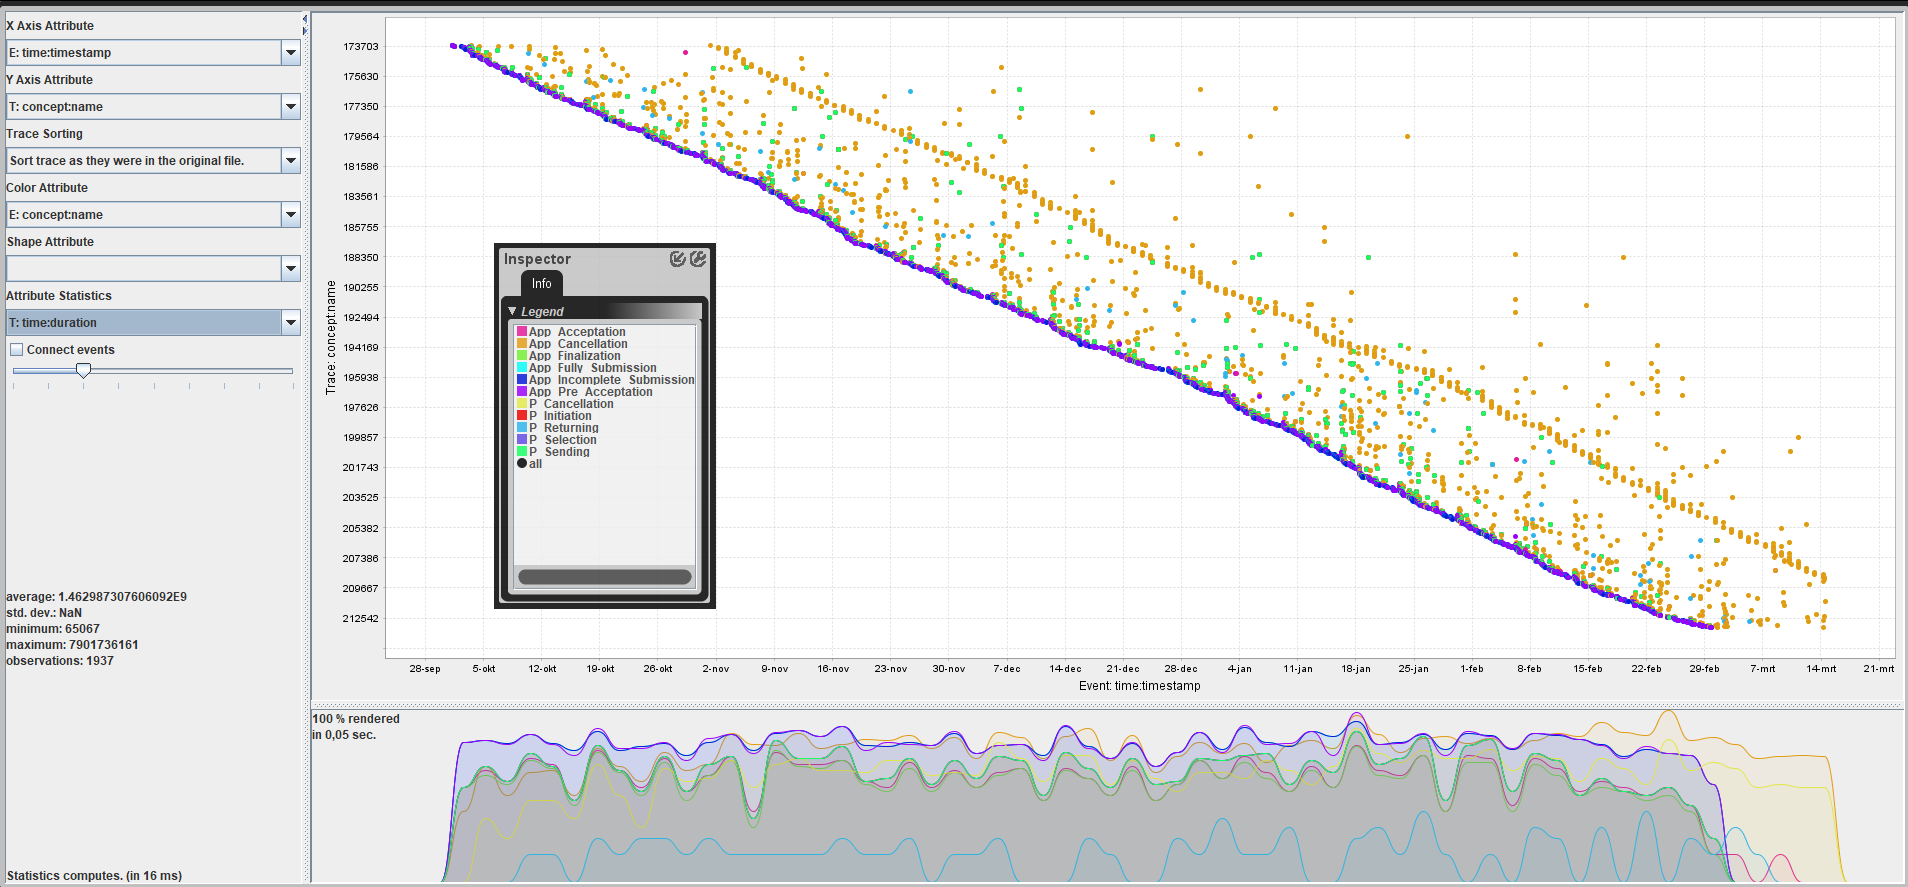
\includegraphics[height = 0.2\textheight]{CancDot.PNG}
\caption{Dotted chart showing the time of events}
\label{fig:CancTimeFlow}
\end{figure}

In figure \ref{fig:CancTimeFlow} the corresponding dotted chart can be seen. On every sunday there are just two events executed "App\_Pre\_Acceptation" and "App\_Incomplete\_Submission". Furthermore in the left lower corner the following information can be found: the average duration of a case is, 16 days 22 hours 23 minutes and 7.31 seconds, the minimal duration, 1 minute and 5.067 seconds, and the maximum duration, 90 days 3 hours 48 minutes and 38.29 seconds. All three values are given in milliseconds in the figure.

There are 11 different events (relative occurences):
"App\_Cancellation" (14.323\%), "App\_Fully\_Submission" (14.323\%), "App\_Incomplete\_Submission" (14.323\%), "App\_Pre\_Acceptation" (14.315\%), "P\_Cancellation" (7.572\%), "P\_Initiation" (7.572\%), "P\_Sending" (7.572\%), "P\_Selection" (7.572\%), "App\_Acceptation" (6.182\%), "App\_Finalization" (5.694\%) and "P\_Returning" (0.555\%). There are 46 different variants of traces.

All traces start with "App\_Fully\_Submission"

A maximum of 32 events is executed in a case and minimal 3. The mean of events per class is 6.982.


\textbf{Discover and evaluate models of lifecycle with Endstate APP\_Cancelled}

\begin{figure}[!htbp]
\centering
\begin{tabular}{c|c|c|c|}
\cline{2-4}
& \multicolumn{3}{ c| }{Frequency} \\ \cline{2-4}
& 0 & 0.049 & 0.1 \\ \cline{1-4}
\multicolumn{1}{ |c|  }{Simplicity} 
& - & + & ++      \\ \cline{1-4}
\multicolumn{1}{ |c|  }{Fitness}  & 99.96 & 99.39 & 96.84       \\ \cline{1-4}
\multicolumn{1}{ |c| } {Precision} & 92.5 & 91.8 & 94.6   \\ \cline{1-4}
\end{tabular}
\caption{Results for cancelled as endstate}
\label{tab:CancRe}
\end{figure}
Like for APP\_Approved I checked different configurations and based on the results, \ref{tab:CancRe}, I decided to pick 0.1 filtered frequency model. The fitness and precision is still higher than 90\%, but it is also the most simpel model.

\textbf{Discussion of the model}

\begin{figure}[!htbp]
\centering
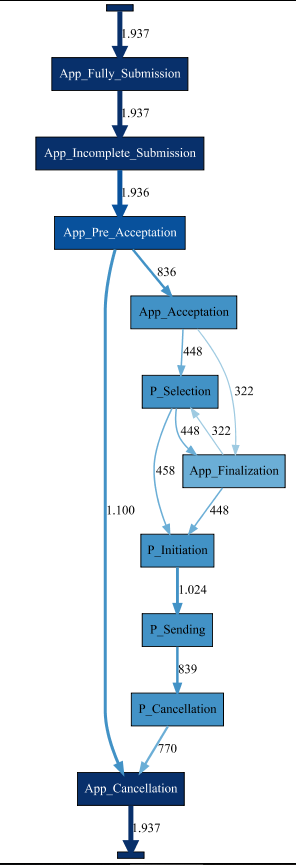
\includegraphics[width=0.9\textwidth]{APP_CancDFG0-1.PNG}
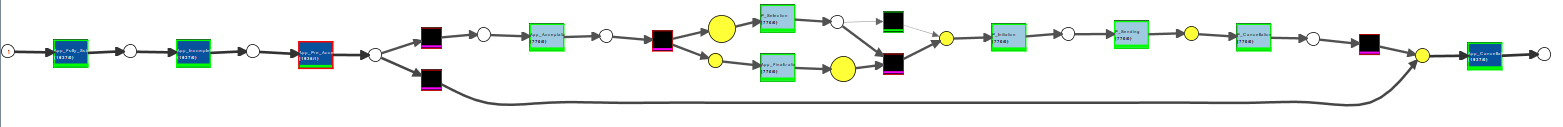
\includegraphics[width=0.9\textwidth]{CancReplay.PNG}
\caption{Endstate APP\_Cancelled}
\label{fig:CancModel}
\end{figure}

In figure \ref{fig:CancModel} the petri net and the result of the replay can be seen.

All cases start with "App\_Fully\_Submission" \textrightarrow "App\_Incomplete\_Submission" \textrightarrow "App\_Pre\_Acceptation" (this is just executed in 1936 cases). Then in 1167 cases "App\_Cancellation" follows directly. Otherwise "App\_Acceptation" (770 cases), followed by "P\_Selection" and "App\_Finalization" in random order. After those are executed, "P\_Initiation" \textrightarrow "P\_Sending" \textrightarrow "P\_Cancellation" \textrightarrow"App\_Cancellation" is executed.

The time transition matrix showed me, that the transition to "App\_Finalization" and "P\_Cancellation" took the most time (between 17 and 22.5 days).


\subsubsection{Endstate APP\_Rejected}

\textbf{General Details of the data set}

The data set was collected between the 1st of 0ct 2011 (saturday), 08:11:08 and the 14th of Mar 2012 (Wednesday), 15:20:23. The set contains 7252 and 26691 events executed. 

\begin{figure}[!htbp]
\centering
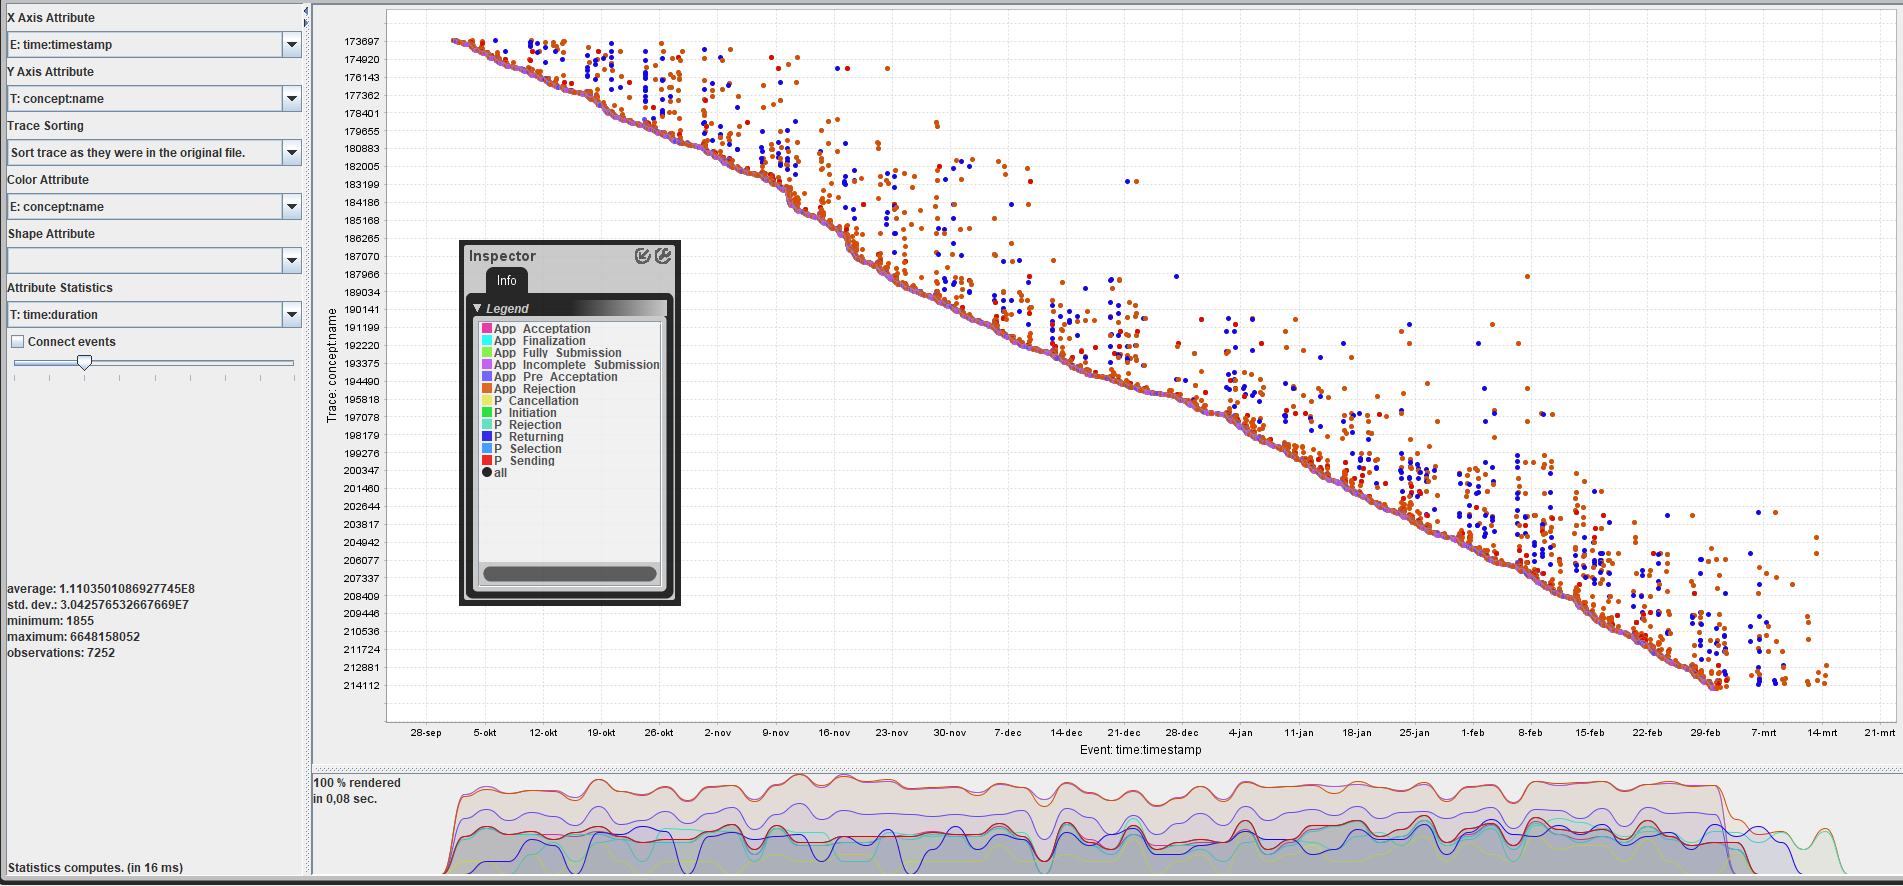
\includegraphics[height = 0.2\textheight]{RejDot.PNG}
\caption{Dotted chart showing the time of events}
\label{fig:RejTimeFlow}
\end{figure}

In figure \ref{fig:RejTimeFlow} the dotted chart can be seen. On every sunday there are just two events executed "App\_Rejection" and "App\_Incomplete\_Submission". Furthermore in the left lower corner the following information can be found: the average duration of a case is, 1 days 6 hours 50 minutes and 35.01 seconds, the minimal duration, 1.855 seconds, and the maximum duration, 76 days 22 hours 42 minutes and 38.05 seconds. All three values are given in milliseconds in the figure.

There are 12 different events (relative occurences):
"App\_Rejection" (27.17\%), "App\_Fully\_Submission" (27.17\%), "App\_Incomplete\_Submission" (27.17\%), "App\_Pre\_Acceptation" (5.744\%), "P\_Initiation" (1.997\%), "P\_Sending" (1.997\%), "P\_Selection" (1.997\%), "App\_Acceptation" (1.678\%), "App\_Finalization" (1.57\%), "P\_Rejection" (1.57\%), "P\_Returning" (1.51\%), "P\_Cancellation" (0.427\%). There are 30 different variants of traces.

All traces start with "App\_Fully\_Submission"

A maximum of 12 events is executed in a case and minimal 3. The mean of events per class is 3.681.


\textbf{Discover and evaluate models of lifecycle with Endstate APP\_Rejected}

The last analysis is of the models ending in APP\_Rejected. In the first step I checked different frequency filters and decided based on simplicity and traceability I had to take a closer look at 0, 0.025 and 0.1.

\begin{figure}[!htbp]
\centering
\begin{tabular}{c|c|c|c|}
\cline{2-4}
& \multicolumn{3}{ c| }{Frequency} \\ \cline{2-4}
& 0 & 0.025 & 0.1 \\ \cline{1-4}
\multicolumn{1}{ |c|  }{Simplicity} 
& - & + & +++      \\ \cline{1-4}
\multicolumn{1}{ |c|  }{Fitness}  & 1.00 & 99.60 & 96.91       \\ \cline{1-4}
\multicolumn{1}{ |c| } {Precision} & 99.3 & 98.7 & 100   \\ \cline{1-4}
\end{tabular}
\caption{Results for cancelled as endstate}
\label{tab:RejRe}
\end{figure}

Based on \ref{tab:RejRe} I chose 0.1 filtered frequency model as the best. It is really easy to follow and has a good fitness.

\textbf{Discussion of the model}

\begin{figure}[!htbp]
\centering
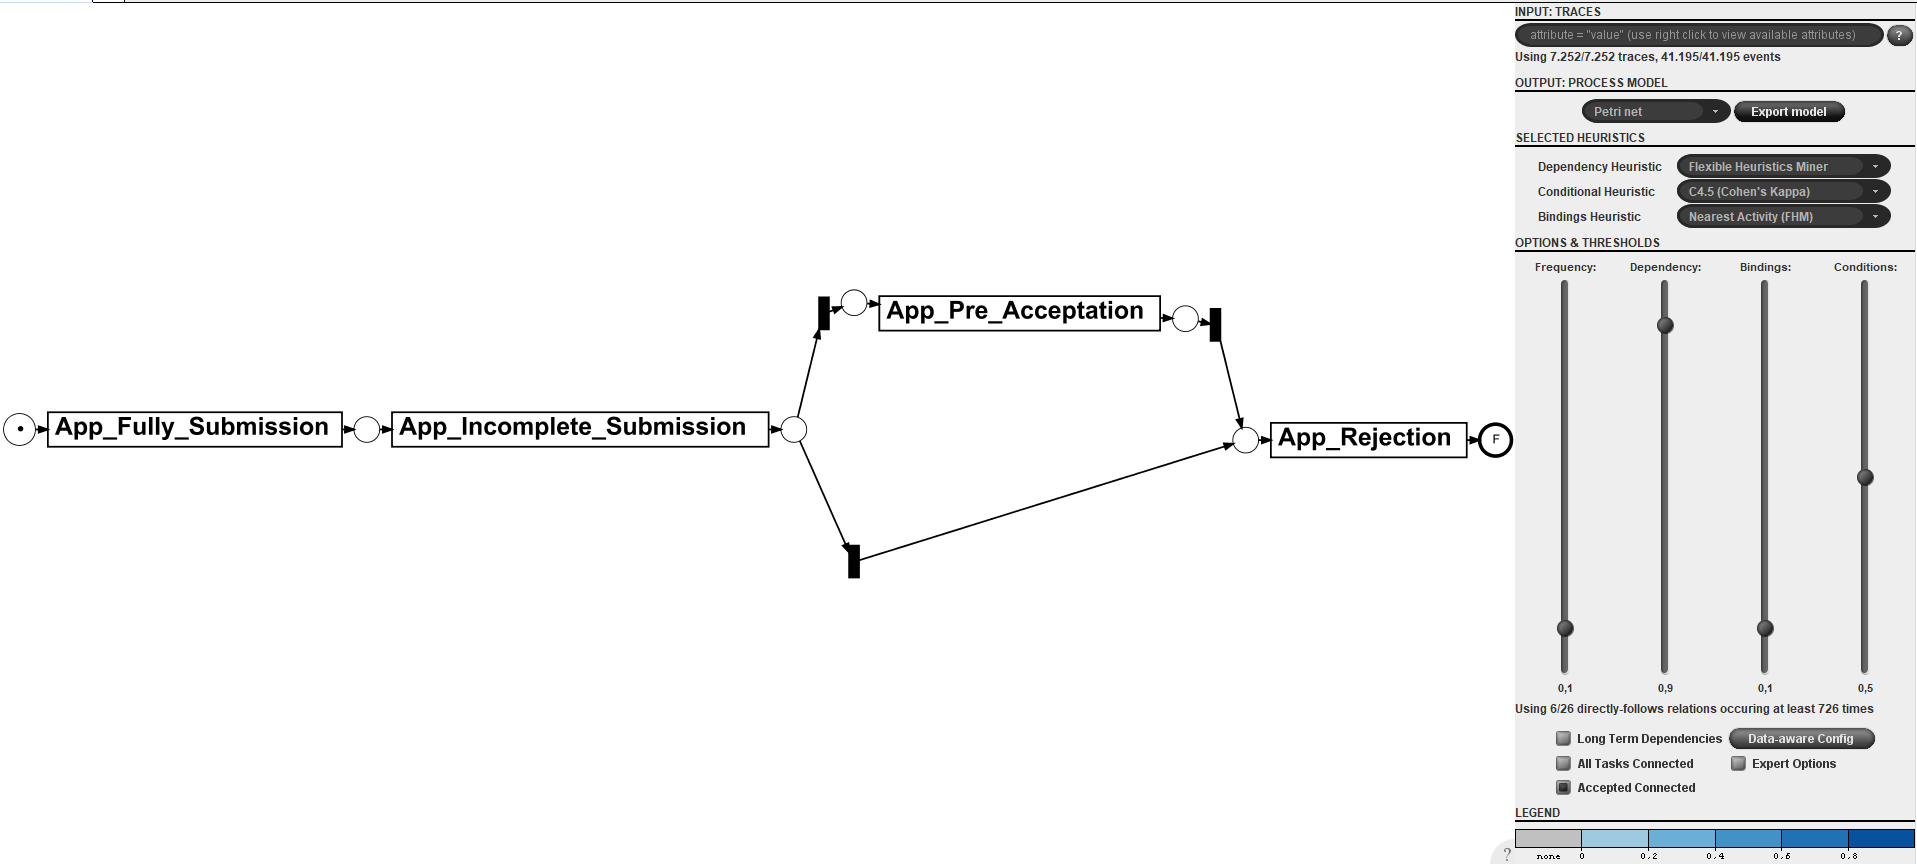
\includegraphics[width=0.9\textwidth]{Rej0-1.PNG}
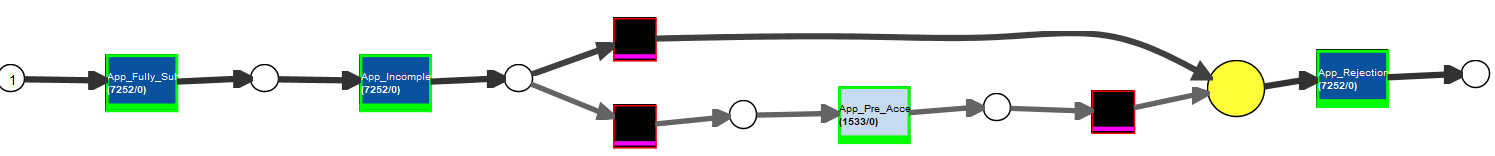
\includegraphics[width=0.9\textwidth]{RejReplay.PNG}
\caption{Endstate APP\_Rejected}
\label{fig:RejModel}
\end{figure}

In figure \ref{fig:RejModel} the model and the replay can be seen. 

The process starts with "App\_Fully\_Submission" \textrightarrow "App\_Incomplete\_Submission" (7252 cases). This is or followed directly by "App\_Rejection" (5719 cases) or first by "App\_Pre\_Acceptation" (1533 cases) and then "App\_Rejection". No details presented for "App\_Rejection" due to filtering.

The worst transition is with 5.51 days from "App\_Pre\_Acceptation" to "App\_Rejection".

\subsection{C-net of the proposal process}
%Analyze the C-net of the proposal process and explain it. 

Based on the results of my analysis of the model before I chose the same frequency filtering for the C-net of the proposal process.
\begin{figure}[!htbp]
\centering
\begin{subfigure}{0.3\textwidth}
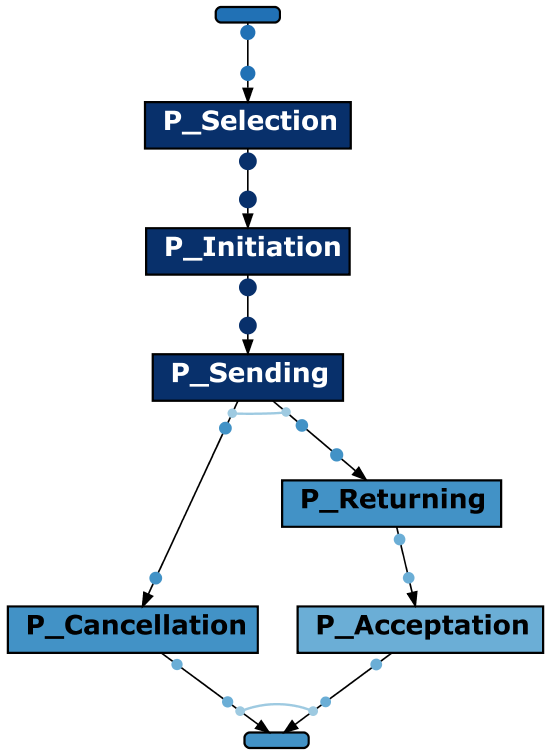
\includegraphics[height = 0.2\textheight]{PCnet0-2.PNG}
\caption{C-net with 0.2 filtered frequency}
\label{fig:cnetP0-2}
\end{subfigure}
\begin{subfigure}{0.7\textwidth}
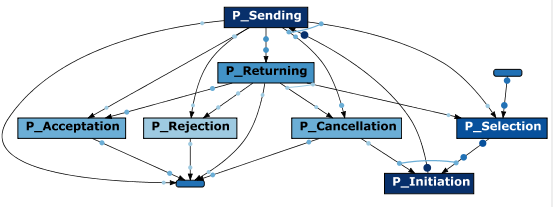
\includegraphics[height = 0.2\textheight]{PropC-Net0.PNG}
\caption{C-net without filtered frequency}
\label{fig:cnetP0}
\end{subfigure}
\caption{C-Nets of the proposal process}
\label{fig:cNetP}
\end{figure}

In figure \ref{fig:cNetP} I show two C-nets of the proposal process for comparsion. \ref{fig:cnetP0-2} is the one I picked and I will discuss in detail. In \ref{fig:cnetP0} the original C-net of the process is to see and obviously it is much more complicated and not so intuitive than the filtered one. 

\subsubsection{Analysis of the C-net}
For simplicity reasons I will not write "P\_" as prefix of every activity.

The first thing I did is having a look at the maximum number of bindings. This is for sending with 3 possible bindings. The input is always from initiation, but there are 3 different outputs possible.
All trace possibilities:
\begin{figure}[!htbp]
\begin{itemize}
	\item Selection \textrightarrow Initiation \textrightarrow Sending \textrightarrow
	\begin{itemize}
	\item  Returning \textrightarrow Acceptation \textrightarrow Done
	\item Cancellation \textrightarrow Returning \textrightarrow Acceptation \textrightarrow Done
	\item  Returning \textrightarrow Acceptation \textrightarrow Cancellation  \textrightarrow Done
	\item  Returning \textrightarrow Cancellation \textrightarrow Acceptation \textrightarrow Done
	\item Cancellation \textrightarrow Done
	\end{itemize}
\end{itemize}
\end{figure}

These 5 pathes are also what you would expect a little bit, but you clearly see, that there are missing details. But depending on the further results those pathes are the main pathes.

\subsubsection{Extra C-net}

\begin{figure}[!htbp]
\centering
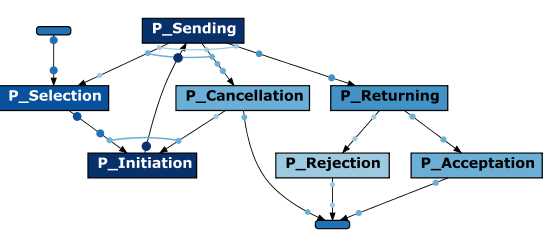
\includegraphics[width=0.9\textwidth]{PropC-Net0-151.PNG}
\caption{C-net with 0.151 filtered frequency}
\label{fig:cnet0-151}
\end{figure}

Just for comparsion I also checked the 0.151 filtered c-net and there you can see, that in real data a loop can be found between Sending, Cancellation, Initiation and Selection. So this behaviour makes the processes probably slower.

\subsection{Own Petri net of the proposal process}
%Based on your analysis, create a Petri net of the proposal process by your own. For example, do not consider infrequent paths and also outlier behaviors. 
Based on my analysis of the C-net and also the petri net.The first problem I saw, was that the start event can occur in between again. Because of that you have a deadlock if you would build it without transitions, that can occur more than once. Also the cancellation and selection or just cancellation or split makes problems. 

Then just checking the different variants and the occurences I found out, that already just the traces occur at least 1\% of the time have "P\_Selection" as start state and as in between state. So I decided just to emphasize the main three main variants. I think this is the behaviour as it should be.

The traces that I considered were:

"P\_Selection"\textrightarrow "P\_Intiation" \textrightarrow "P\_Sending"\textrightarrow
\begin{itemize}
	\item "P\_Returning" \textrightarrow "P\_Acceptation" (1.537 cases, 11.74\%)
	\item "P\_Returning" \textrightarrow "P\_Rejection" (1.132 cases, 8.65\%)
	\item "P\_Cancellation" (574 cases, 4.39\%)
\end{itemize}


\begin{figure}[!htbp]
\centering
\begin{tikzpicture}[node distance=1.5cm,>=stealth',bend angle=45,auto]

  \tikzstyle{place}=[circle,thick,draw=blue!75,fill=blue!20,minimum size=6mm]
  \tikzstyle{transition}=[rectangle,thick,draw=black!75,
  			  fill=black!20,minimum size=4mm]

  \tikzstyle{every label}=[red]

  \begin{scope}
    % First net
    \node [place,tokens=1] (start)                {};
    \node [transition] (selection) [right of=start]       {Selection}
    	edge [pre] (start);
    \node [place] (tos)  [right of=selection]	  	  {}
    	edge [pre] (selection);
    \node [transition] (initiation) [right of=tos]         {Initiation}
    	edge [pre] (tos);
    \node [place] (itos) [right of=initiation] {}
    	edge [pre] (initiation);
    \node [transition] (sending) [right of=itos] {Sending}
    	edge [pre] (itos);
    \node [place] (storc) [right of=sending] {}
    	edge [pre] (sending);
    \node [transition] (returning) [right of=storc] {Returning}
    	edge [pre] (storc);
    \node [place] (rtoar) [right of=returning] {}
    	edge [pre] (returning);
    \node [transition] (acceptation) [below of=rtoar] {Acceptation}
    	edge [pre] (rtoar);	
    \node [place] (end) [right of=acceptation] {}
    	edge [pre] (acceptation);
    	%edge [pre] (cancellation)
    	%edge [pre] (rejection);
    \node [transition] (rejection) [above of=rtoar] {Rejection}
    	edge [post] (end)
    	edge [pre] (rtoar);
    \node [transition] (cancellation) [below of=acceptation] {Cancellation}
    	edge [pre] (storc)
    	edge [post] (end);
    %\node [place] (end) [right of=acceptation] {}
    %	edge [pre] (acceptation)
    %	edge [pre] (cancellation)
    %	edge [pre] (rejection);
  \end{scope}
\end{tikzpicture}
\caption{Own petri-net}
\label{pet:Own}
\end{figure}



\subsection{Analysis of the performance of Application and work process}
%Analyze the performance of Application and work process. What are the bottlenecks? What are your recommendations to the company to increase the performance of the process? 

Just the events beginning with "App\_..." or "W\_..." are required. The resulting data set is saved as "Filtered Work and App". I also just considered the workdataset (data beginning with "W\_..") saved as "Filtered Work"

\subsubsection{General Details of the data set}
The data set is collected between the 1st of 0ct 2011 (saturday), 00:38:44 and the 14th of Mar 2012 (Wednesday), 16:04:54 and contains 13087 cases with 230956 events. 

\begin{figure}[!htbp]
\centering
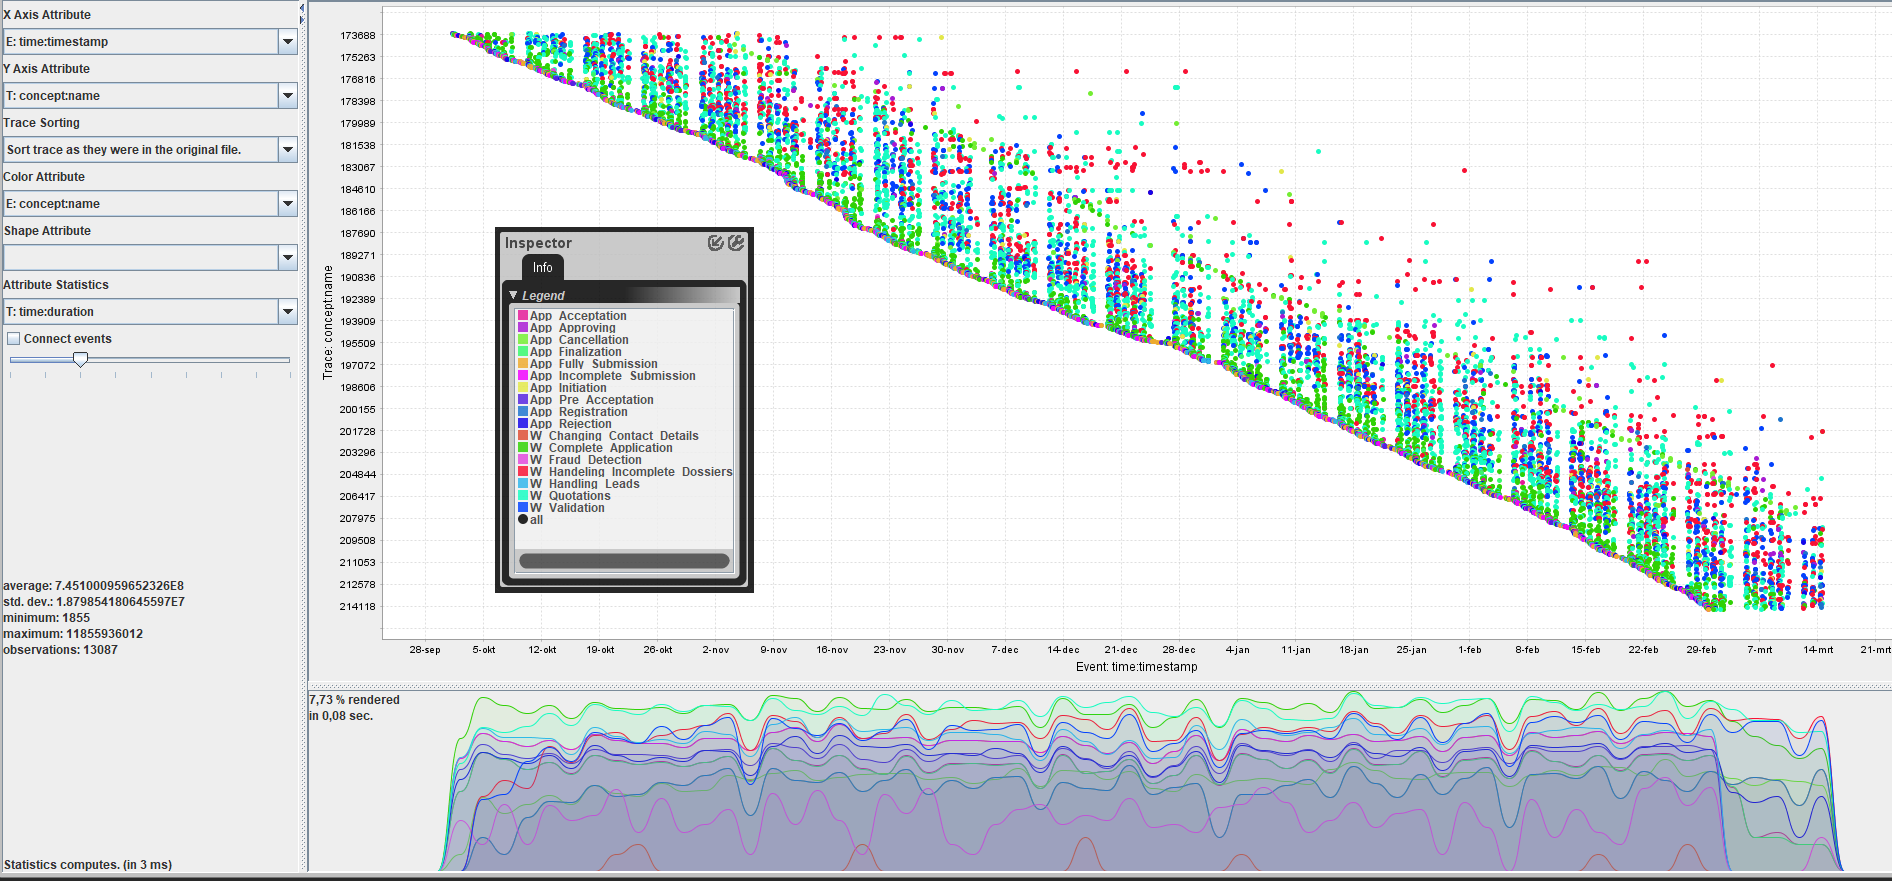
\includegraphics[width = 0.8\textwidth]{AppWorkDot.PNG}
\caption{Dotted chart showing the time of events}
\label{fig:AppWorkTimeFlow}
\end{figure}

In figure \ref{fig:AppWorkTimeFlow} the dotted chart can be seen. Having a closer look at this I saw again gaps on sunday. On sundays just "App\_Incomplete\_Submission" and "App\_Rejection" is been executed. Furthermore is in the left below corner to see what is the average duration of a case, 8 days 14 hours 58 minutes and 20.10 seconds, the minimum duration, 13.087 seconds, and the maximum duration, 137 days 5 hours 18 minutes and 56.01 seconds. Both is given in milliseconds.

The data set has 29 events (occurence relative): 
"W\_Complete\_Application" (10.377\%), "W\_Complete\_Application" (10.18\%), "W\_Quotations" (9.948\%), "W\_Quotations" (9.701\%), "App\_Fully\_Submission" (5.666\%), "App\_Incomplete\_Submission" (5.666\%), "W\_Handeling\_Incomplete\_Dossiers" (4.939\%), "W\_Handeling\_Incomplete\_Dossiers" (4.936\%), "W\_Validation" (3.418\%), "W\_Validation" (3.417\%), "App\_Rejection" (3.306\%), "W\_Complete\_Application" (3.192\%), "App\_Pre\_Acceptation" (3.19\%), "W\_Quotations" (2.872\%), "W\_Handling\_Leads" (2.554\%), "W\_Handling\_Leads" (2.553\%), "App\_Acceptation" (2.214\%), "W\_Validation" (2.175\%), "App\_Finalization" (2.171\%), "W\_Handling\_Leads" (2.066\%), "App\_Cancellation" (1.215\%), "W\_Handeling\_Incomplete\_Dossiers" (1.032\%), "App\_Initiation" (0.972\%), "App\_Approving" (0.972\%), "App\_Registration" (0.972\%), "W\_Fraud\_Detection" (0.117\%), "W\_Fraud\_Detection" (0.117\%), "W\_Fraud\_Detection" (0.054\%) and "W\_Changing\_Contact\_Details" (0.005\%).

There are 3668 different variants of traces.

Maximal 162 events are executed in a case and minimal 3. The mean of events per class is 17.648.

All cases start with "App\_Fully\_Submission", but there are 12 different outcomes: 
"App\_Rejection" (26.202\%), "W\_Validation" (20.975\%), "W\_Handling\_Leads" (17.07\%), "W\_Complete\_Application" (14.816\%), "W\_Quotations" (9.895\%), "App\_Cancellation" (7.091\%), "W\_Handeling\_Incomplete\_Dossiers" (3.454\%), "W\_Fraud\_Detection" (0.436\%), "W\_Changing\_Contact\_Details" (0.031\%), "W\_Validation" (0.015\%), "App\_Registration" (0.008\%) and "W\_Quotations" (0.008\%).

\subsubsection{Bottlenecks of the workflow-net}
Using the \textbf{Mine with inductive visual miner} I first explored the workflow process. The configuration were changed to 100\% of the pathes and show paths and sojourn time in the first step.

\begin{figure}[!htbp]
\centering
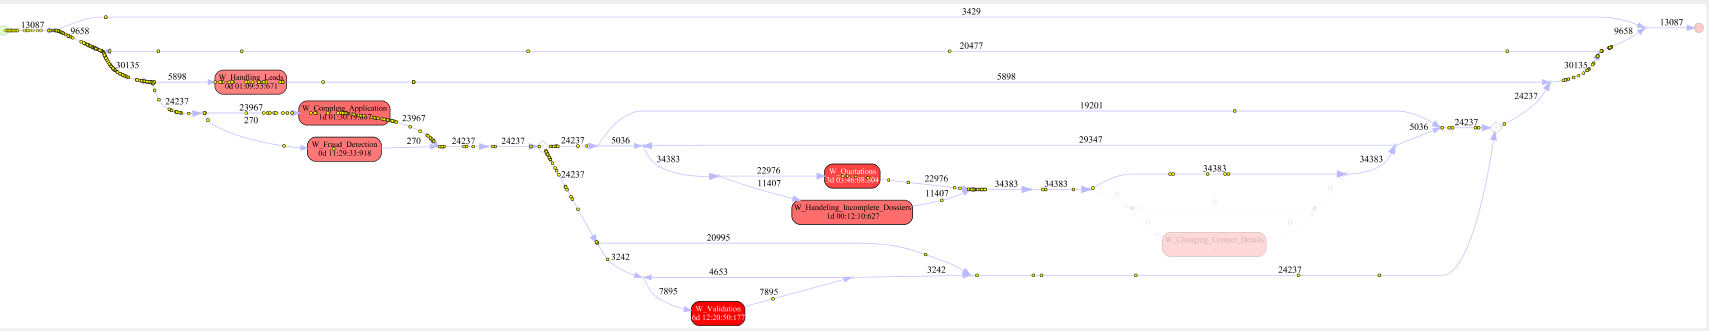
\includegraphics[width = 0.9\textwidth]{WorkSojuComp.PNG}
\caption{Workflow net with sojourn time}
\label{fig: WorkSojuComp}
\end{figure}

The dark red transitions are the transitions with a long preoceeding time, so our searched bottlenecks. The biggest problem we get from the "W\_Validation" step (6 days 12 hours 20 minutes 50 seconds and 177 milliseconds). The second slow trensition is "W\_Quotations" (3 days 3 hours 46 minutes 46 seconds 804 milliseconds). The rest is around 1 day. Having a look at the amount of times the two slow transitions has to be executed it is clear, that "W\_Quotations" makes the process slow. Having a look at the event log visulization you can see, that in the 10 most common processes there are 2, appearing in 1.3\% of the traces, that have at least one time  "W\_Quotations" and they also have "W\_Validation" in it. 

Changing the view to paths and queue lengths and having a look at the longest queues over time I had the same 2 as bottlenecks.

The next thing I controlloed was how many different persons this event can execute, but the result was that both event are executed by 53 for "W\_Quotations" and 54 for "W\_Validation". Conspicuous is, that for "W\_Validation" the first most frequent appearing ressources execute the event in already 57\% of the cases.

\subsubsection{Recommendations based on the workflow-net}

Having a look at the bottlenecks of the workflow-net it can be seen, that for the two bottlenecks a lot of the cases execute the events at least 2 times. This ist obviously to see, because there are just 3242 cases incoming to "W\_Validation", but in total it is executed 7895 times. This make the waiting queue longer and so the overall executing time, too. 

For "W\_Quotations" the problem is similar.

So the first advice I would give is to overthink the procedure in both cases, such that it has to be done just one time, but then on a good manner. Also maybe the workload can be better spreaded if it is not specific or for "W\_Validation" concentrated such that a few people know how to do it and just concentrate on this.


\subsubsection{Bottlenecks of the application-net}
Using the same tool I also had a look at the application process.

\begin{figure}[!htbp]
\centering
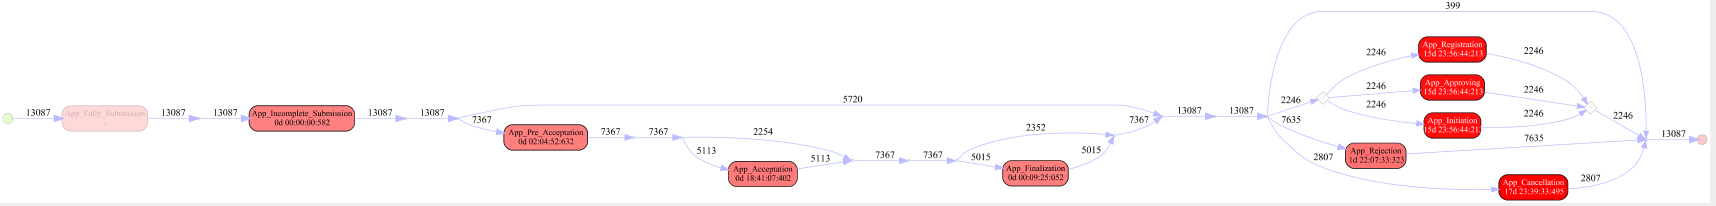
\includegraphics[width = 0.9\textwidth]{AppSojuCom.PNG}
\caption{Application net with sojourn time}
\label{fig: AppSojuComp}
\end{figure}

As to see in figure \ref{fig: AppSojuComp} the most events are done pretty fast, but the events in the end are really slow. 

\begin{figure}[!htbp]
\centering
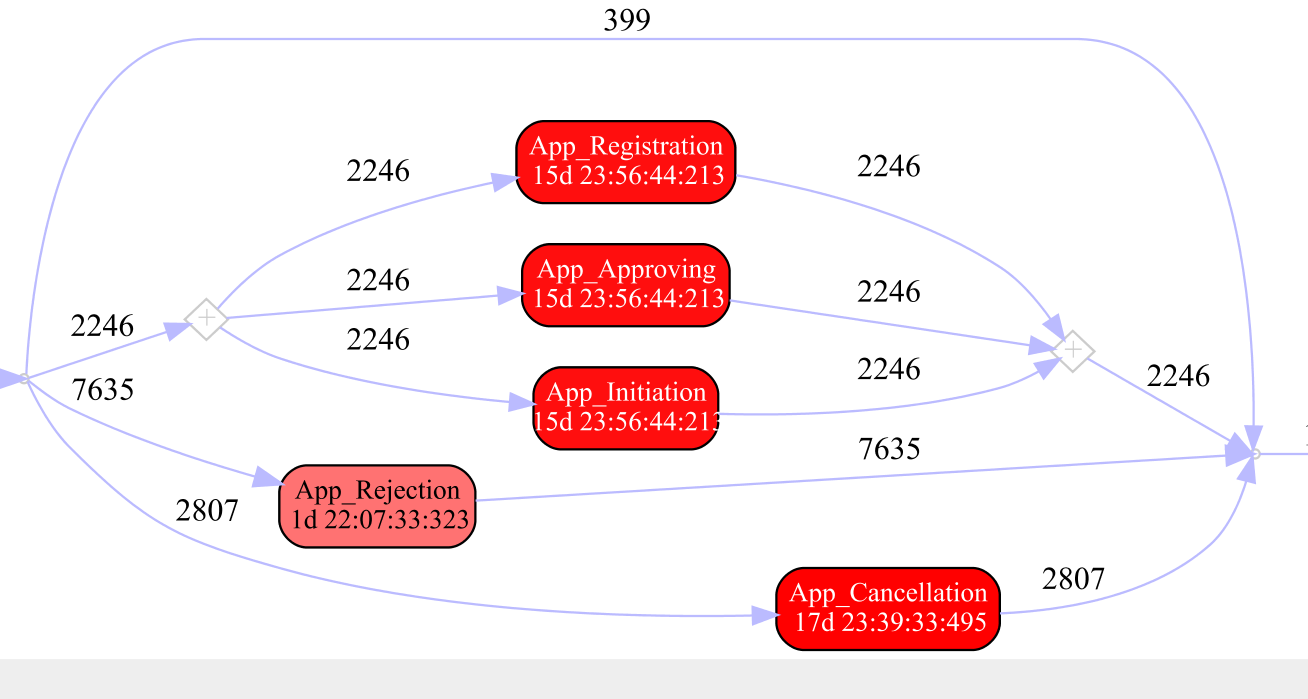
\includegraphics[width = 0.9\textwidth]{AppSojuProb.PNG}
\caption{Zoomed in application net with sojourn time}
\label{fig: AppSojuCompProb}
\end{figure}

Having a closer look at this it can be seen, that the events there take roughly 16 days. "Cancellation" even takes almost 18 days.

Taking a look into the ressources used it is clear, that the work is concentrated on a few persons and not good distributed in between. ("App\_Registration", "App\_Approving", "App\_Initiation" 9 of 61) Just "App\_Cancellation" is done by 58 of 61, but it still takes a high amount of time. Probably, because the peoble are busy with other stuff.

\subsubsection{Recommendations based on the application-net}

Based on the results I would recommend to check, if there is a possibility to accelerate the decision steps. 

\subsubsection{Combined model}

Just to be sure I also executed the process for the complete data set.

\begin{figure}[!htbp]
\centering
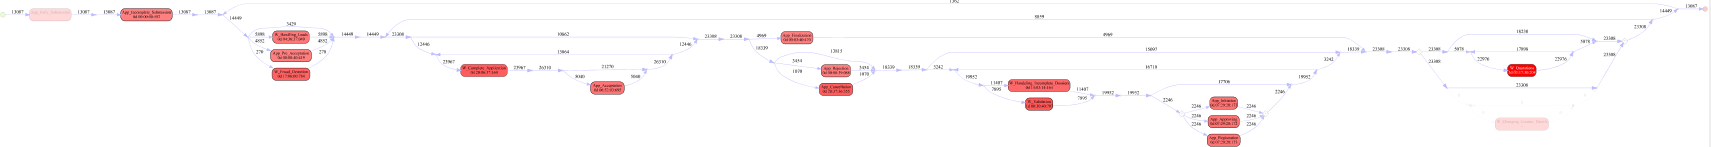
\includegraphics[width = 0.9\textwidth]{APP_Work_Bottle.PNG}
\caption{Application and workflow net with sojourn time}
\label{fig: AppWorkSojuComp}
\end{figure}

In figure \ref{fig: AppWorkSojuComp} the whole net with the sojourn time can be seen. For better understanding I zoomed in at the different critical parts.

\begin{figure}[!htbp]
\centering
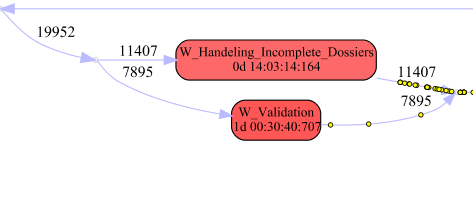
\includegraphics[width = 0.45\textwidth]{APP_Work_BottleVal.PNG}
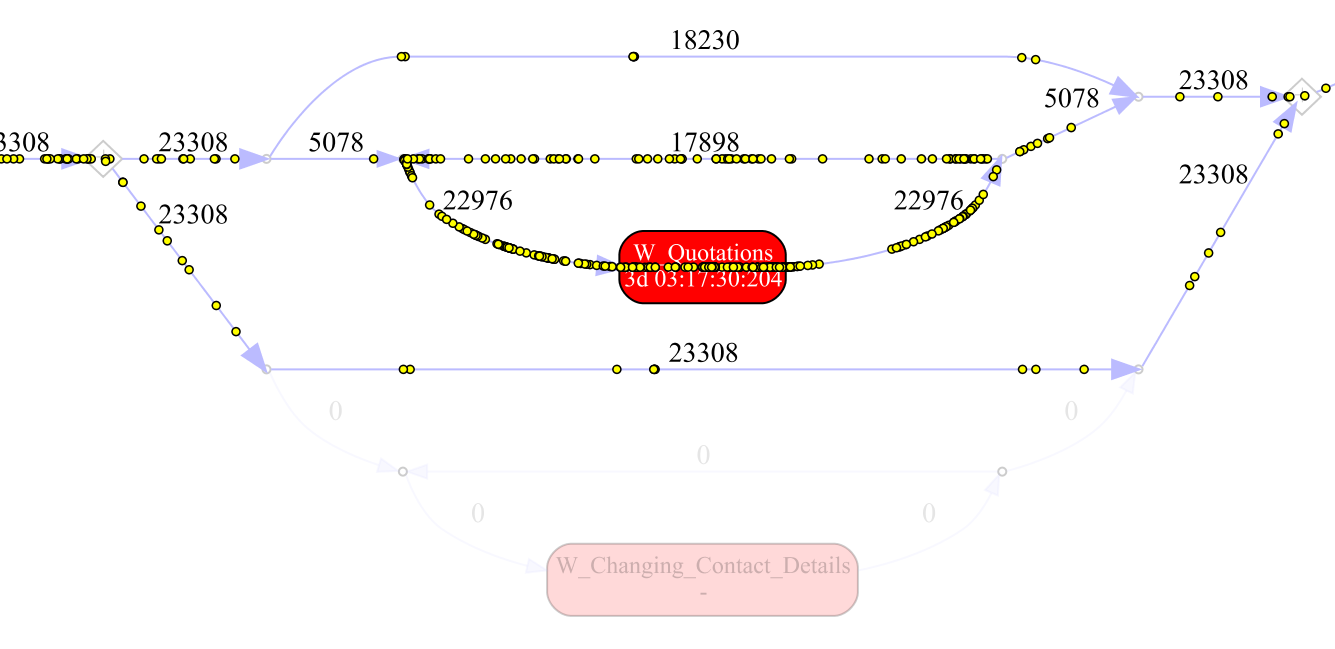
\includegraphics[width = 0.45\textwidth]{APP_Work_BottleQuot.PNG}
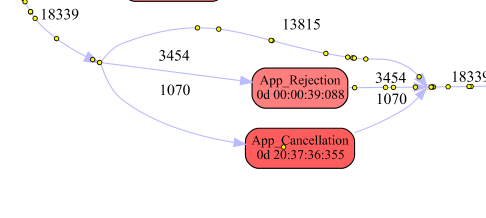
\includegraphics[width = 0.45\textwidth]{APP_Work_BottleCanc.PNG}
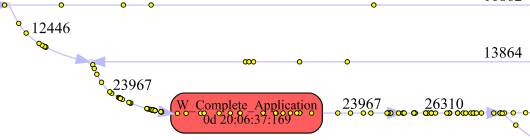
\includegraphics[width = 0.45\textwidth]{APP_Work_BottleCompl.PNG}
\caption{Application and workflow net with sojourn time}
\label{fig: AppWorkSojuComp}
\end{figure}

Like we expected the bottlenecks of the whole net are the same than for the two smaller ones. Just the sojourn times are smaller, because there are more events, that are executed in bettwen and the timestamps are closer to each other. Furthermore it is clear, that the workflow bottlenecks are worde, than the application bottlenecks. The amount of times those events have to be executed is for the workflow events much higher. This clarifys a little bit the high soujoun time, but the process has to be optimized on this parts.

\subsubsection{Recommendations based on the combined net}

Noticeable is, that there are a lot of traces going back and the part has to be executed again. This makes the process slower and also increases the workload for the different steps. So this backloop should be rethinked. 